\documentclass[aspectratio=169, 10pt]{beamer}

% Impostazioni lingua e codifica
\usepackage[utf8]{inputenc}
\usepackage[T1]{fontenc}
\usepackage[italian]{babel}
\usepackage{lmodern}

% Pacchetti matematici, grafici e circuitali
\usepackage{amsmath, amssymb}
\usepackage{booktabs}
\usepackage{graphicx}
\usepackage{circuitikz}
\usepackage{microtype}

% Stile beamer minimale e pulito
\usetheme{default}
\usecolortheme{dove}

% Disattiva simboli di navigazione
\setbeamertemplate{navigation symbols}{}

% Intestazione e piè di pagina minimali
\setbeamertemplate{headline}{}
\setbeamertemplate{footline}{%
  \hfill%
  \usebeamercolor[fg]{page number in head/foot}%
  \usebeamerfont{page number in head/foot}%
  \insertframenumber\,/\,\inserttotalframenumber%
  \kern1.5em\vskip0.8em%
}

% Formattazione del titolo delle slide minimale
\setbeamertemplate{frametitle}{%
  \vspace*{0.3em}%
  \raggedright%
  {\large\color{black!90}\insertframetitle}\par%
  \vspace*{0.1em}%
}

% Spaziature display math compatte
\setlength{\abovedisplayskip}{2pt}
\setlength{\belowdisplayskip}{2pt}
\setlength{\abovedisplayshortskip}{1pt}
\setlength{\belowdisplayshortskip}{1pt}

% Liste senza pallini pesanti
\setbeamertemplate{itemize item}{\raisebox{0.2ex}{\tiny$\bullet$}}
\setbeamertemplate{itemize subitem}{\raisebox{0.2ex}{\tiny$\circ$}}

\title{Caratterizzazione del transitorio elettrico a $V_{DC} = 0\text{ V}$}
\date{}

\begin{document}

% -------------------------------------------------------------
% SLIDE 1: FIT ESPONENZIALE DELL'INVILUPPO DEI PICCHI (4 CASI)
% -------------------------------------------------------------
\begin{frame}{Inviluppo esponenziale dei picchi di oscillazione durante il ring-down}
\centering
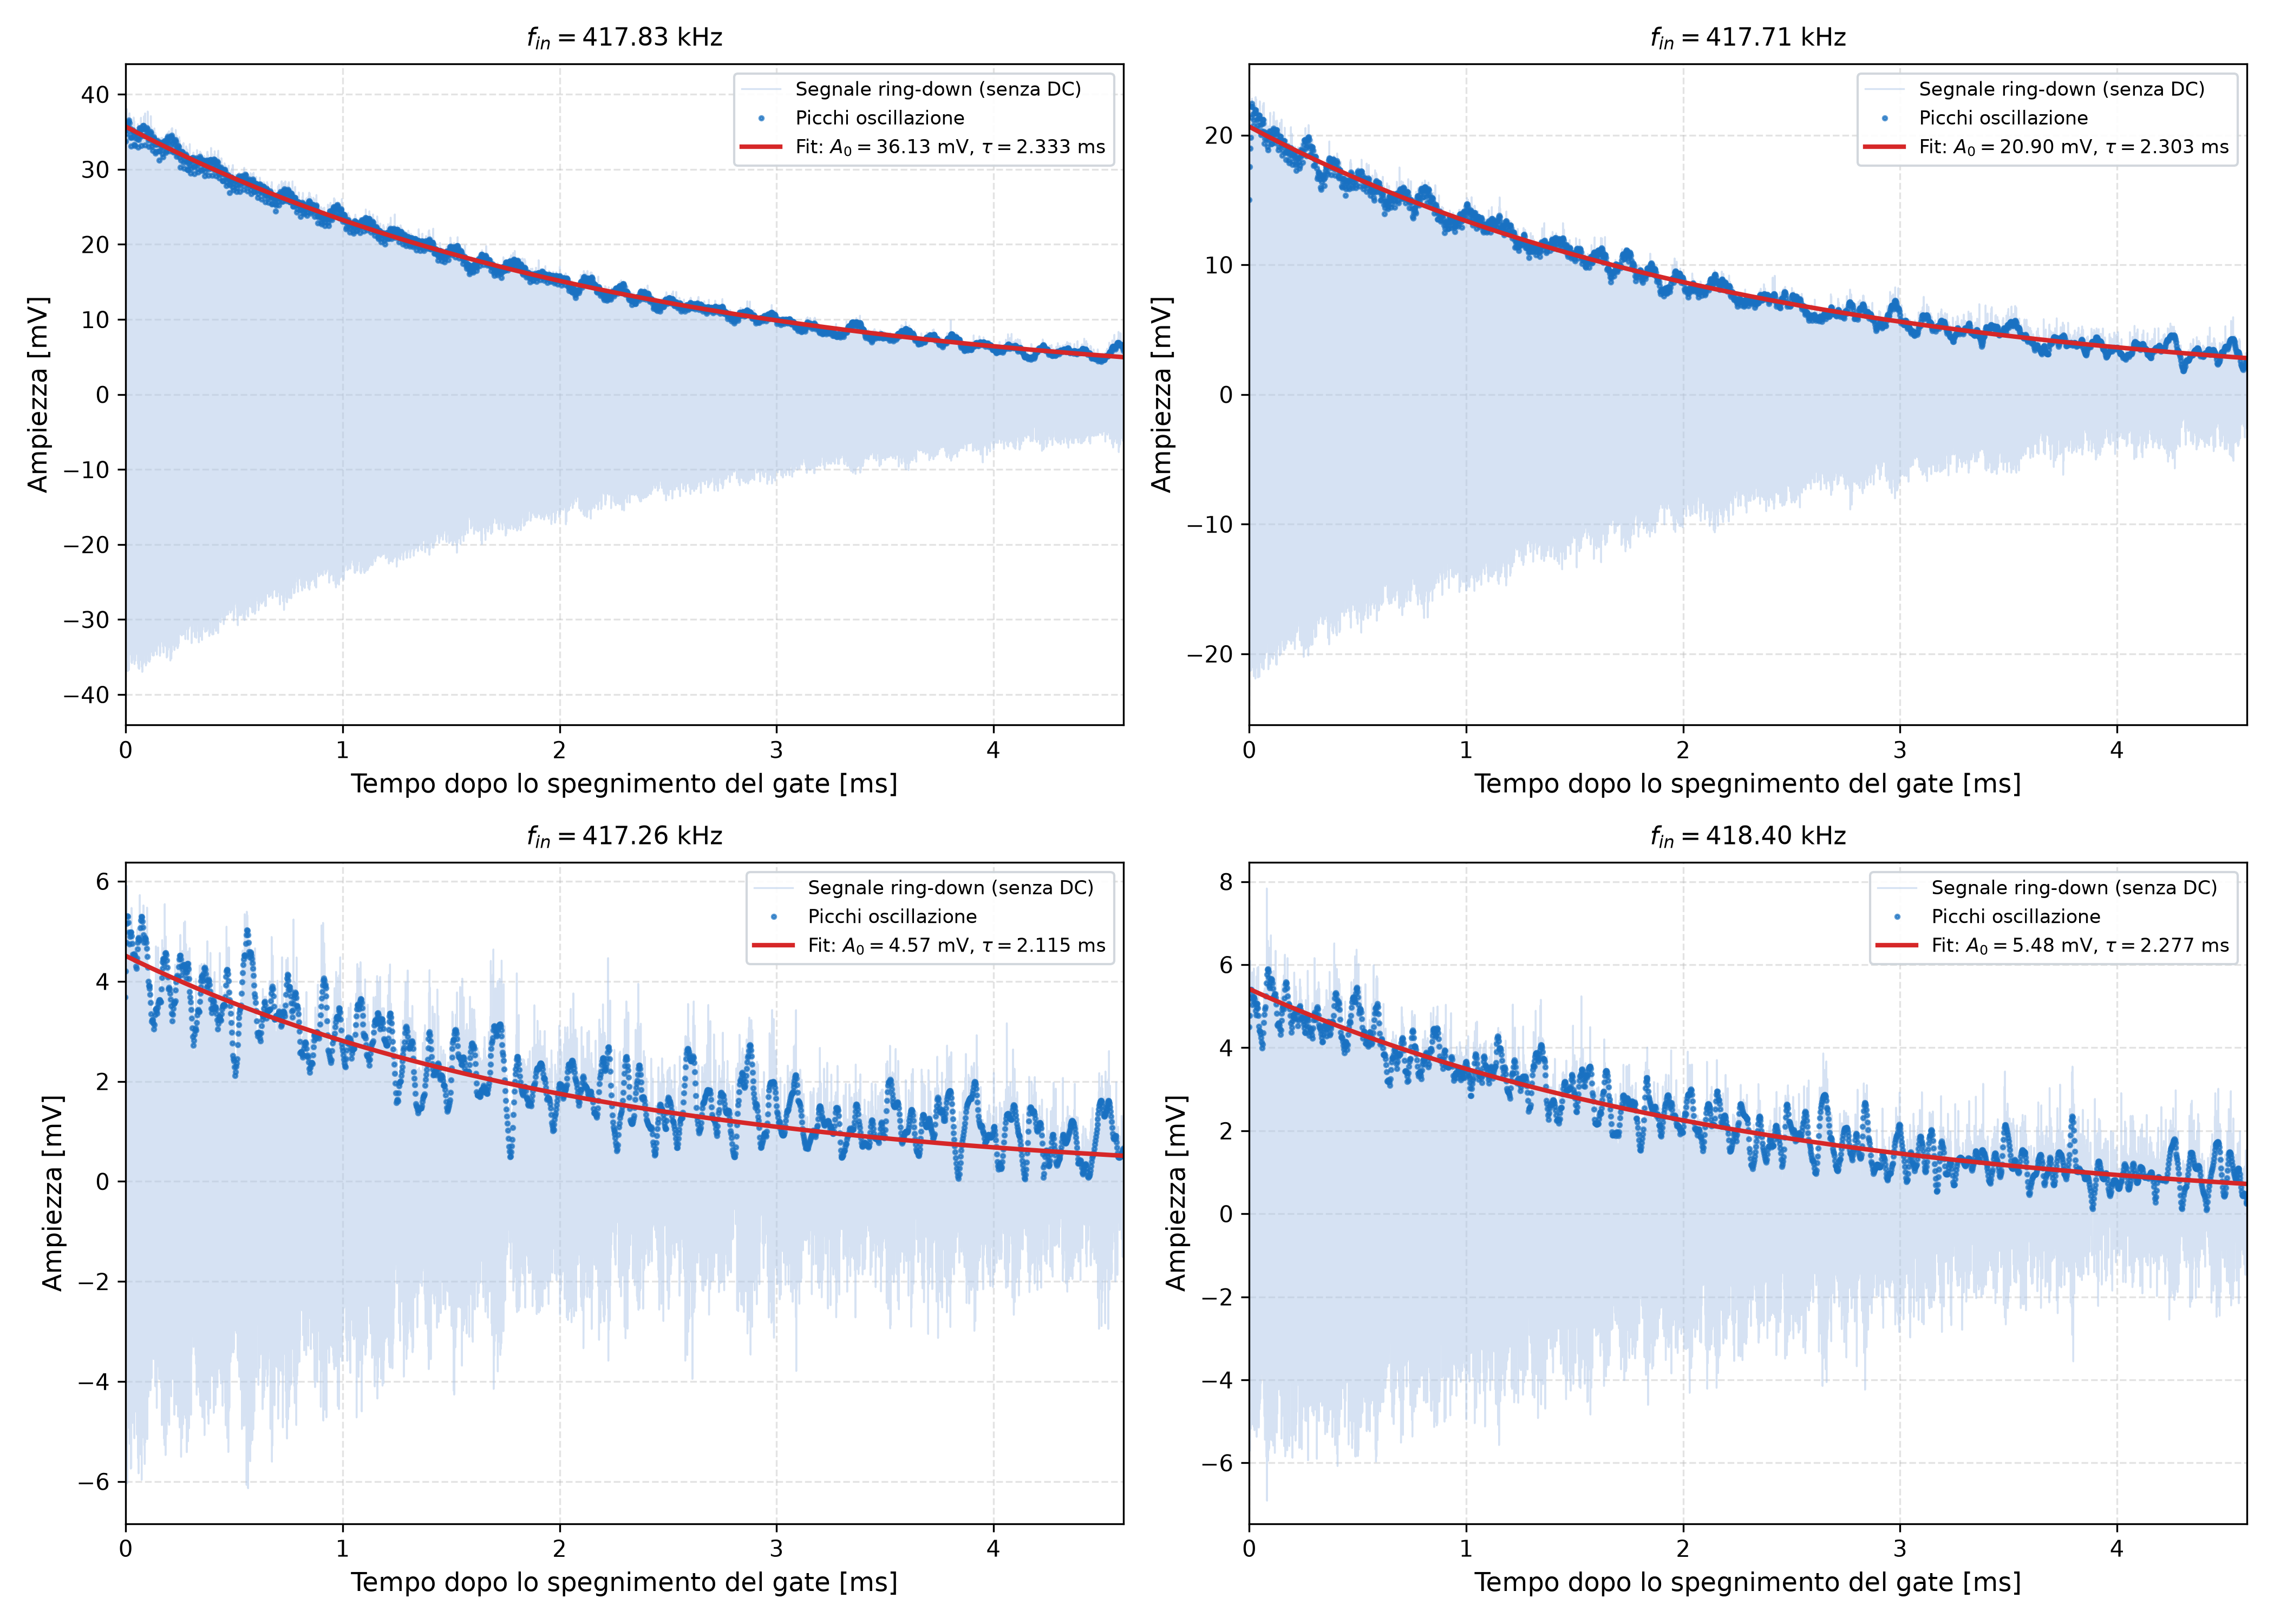
\includegraphics[height=0.78\textheight, width=0.95\textwidth, keepaspectratio]{../Ampiezza_Frequenza/grafici/ringdown_fit_4casi.png}
\end{frame}

% -------------------------------------------------------------
% SLIDE 2: RISPOSTA IN AMPIEZZA DEL MEMS VS FREQUENZA DI INGRESSO
% -------------------------------------------------------------
\begin{frame}
\centering
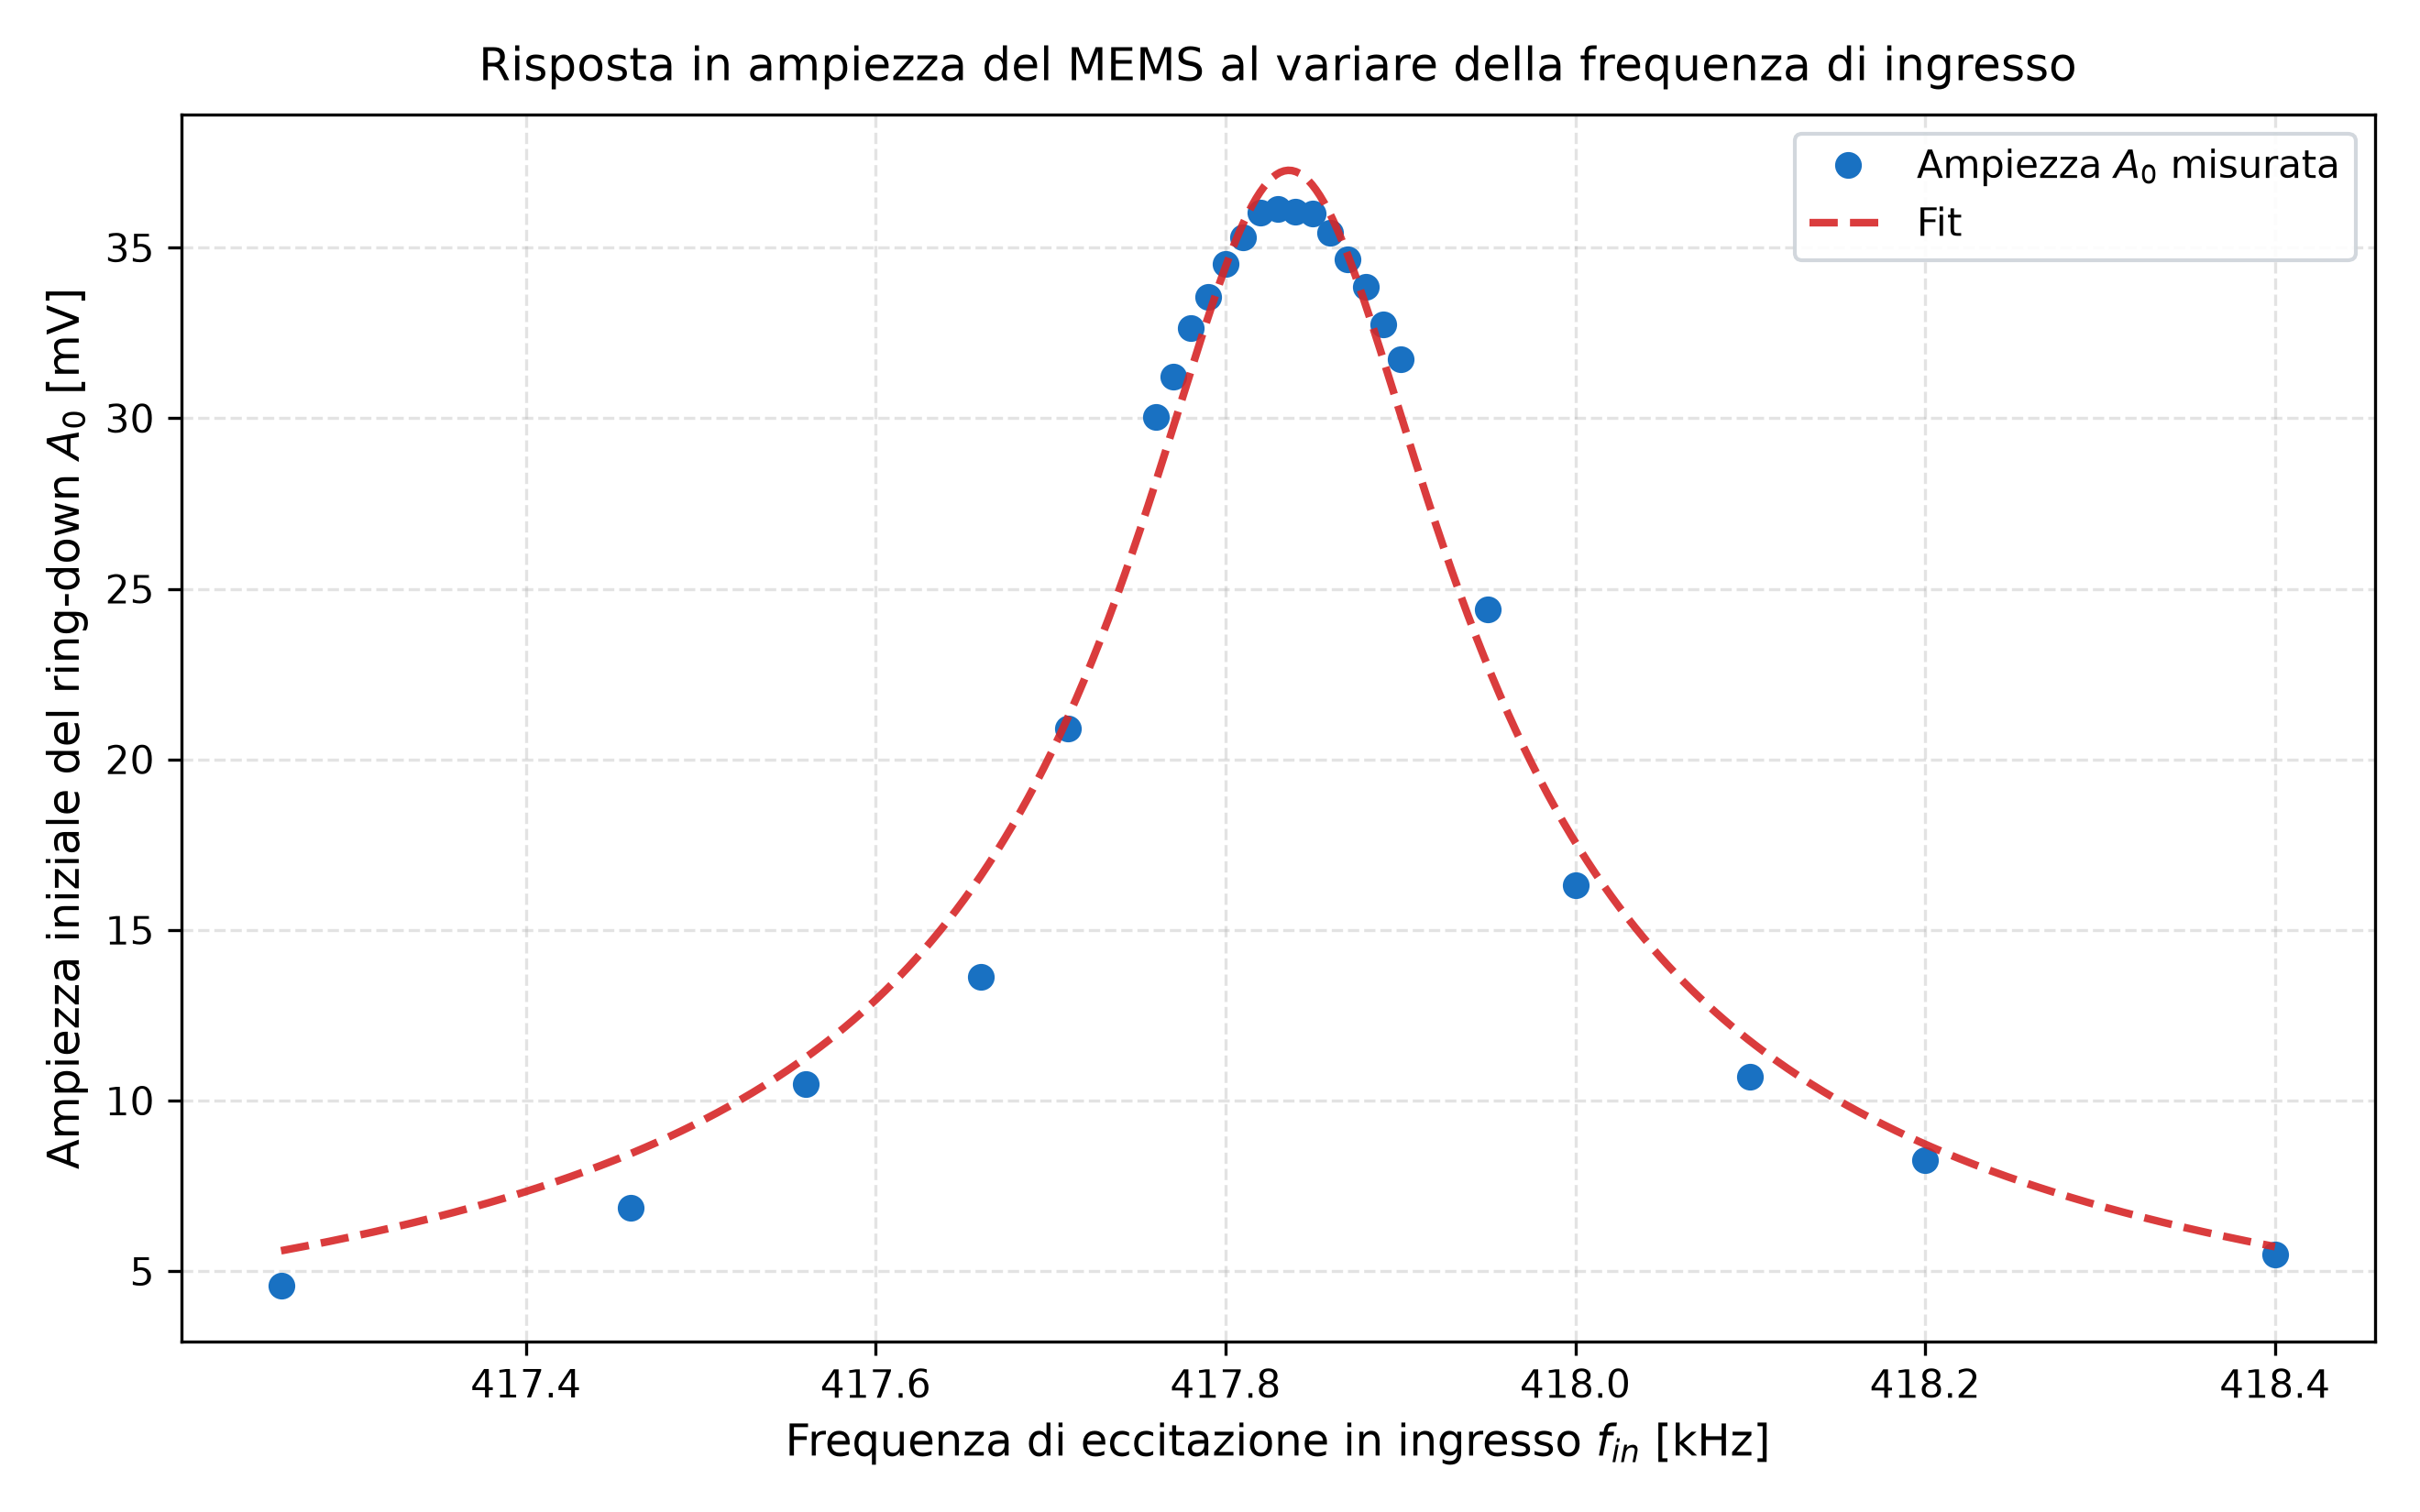
\includegraphics[height=0.88\textheight, width=0.98\textwidth, keepaspectratio]{../Ampiezza_Frequenza/grafici/ampiezza_vs_frequenza.png}
\end{frame}

% -------------------------------------------------------------
% SLIDE 3: FREQUENZA DI OSCILLAZIONE VS FREQUENZA DI INGRESSO
% -------------------------------------------------------------
\begin{frame}
\centering
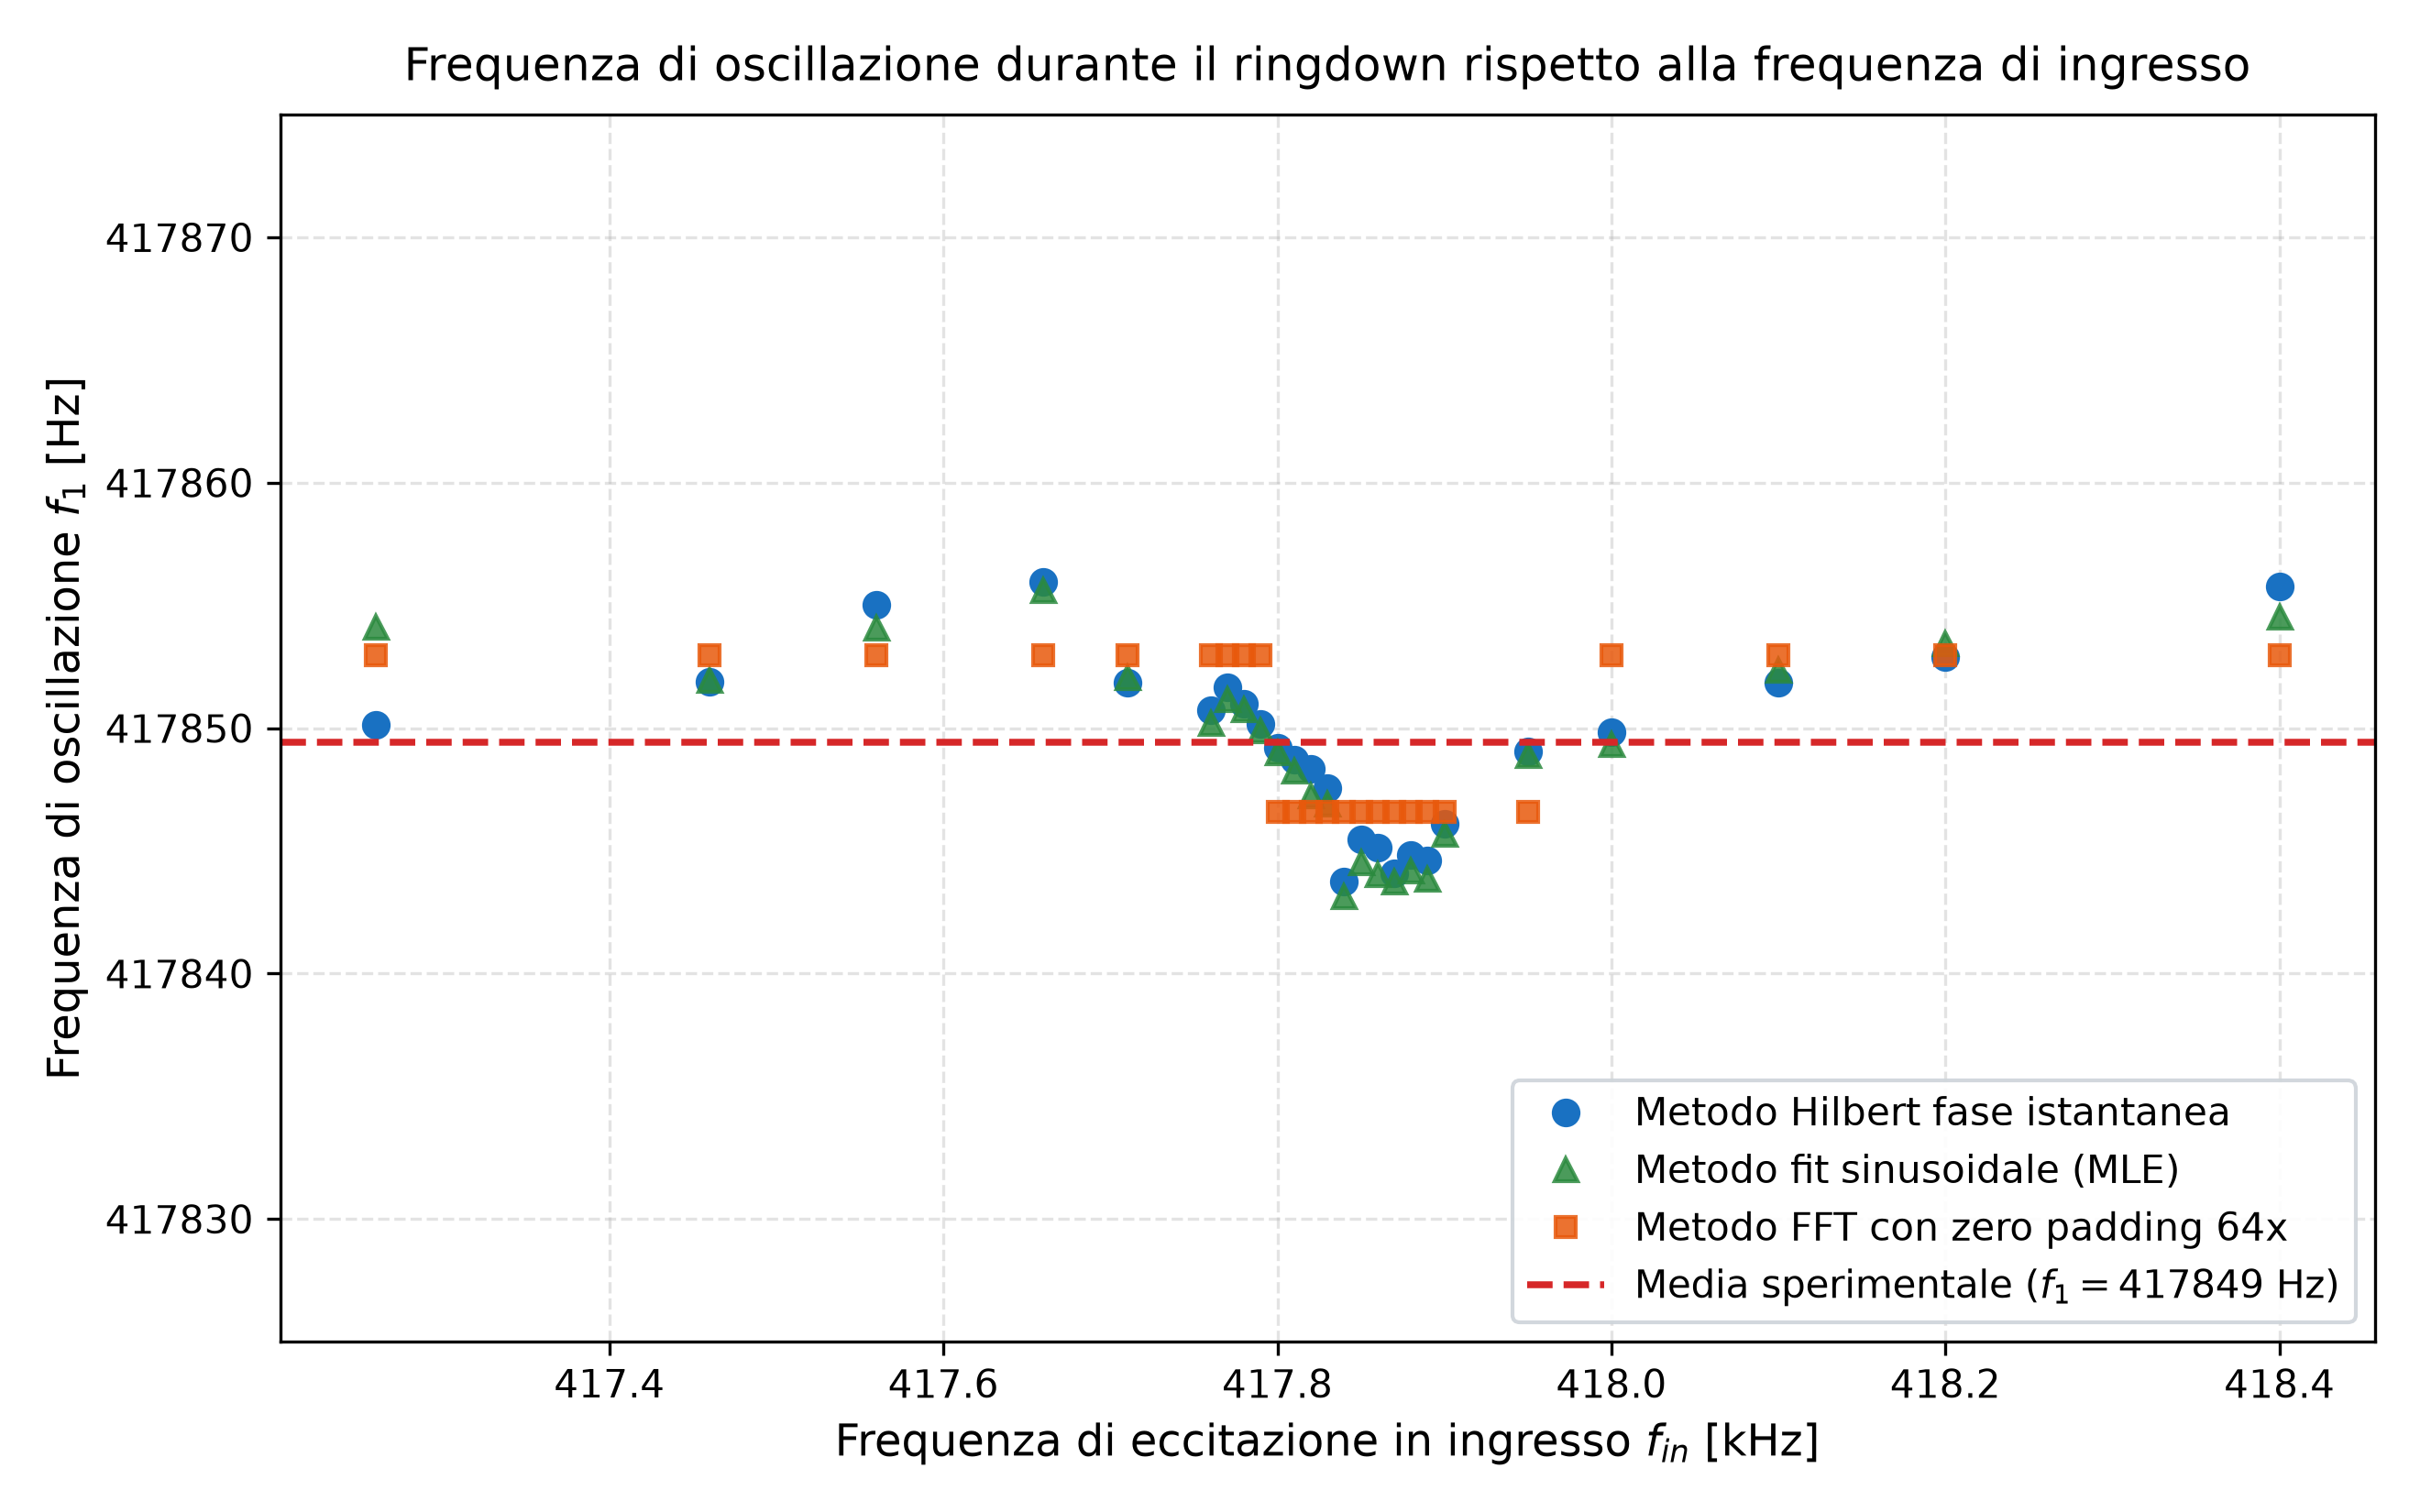
\includegraphics[height=0.88\textheight, width=0.98\textwidth, keepaspectratio]{../Ampiezza_Frequenza/grafici/frequenza_vs_fin.png}
\end{frame}

% -------------------------------------------------------------
% SLIDE 4: COSTANTE DI DECADIMENTO TAU VS FREQUENZA DI ECCITAZIONE
% -------------------------------------------------------------
\begin{frame}
\centering
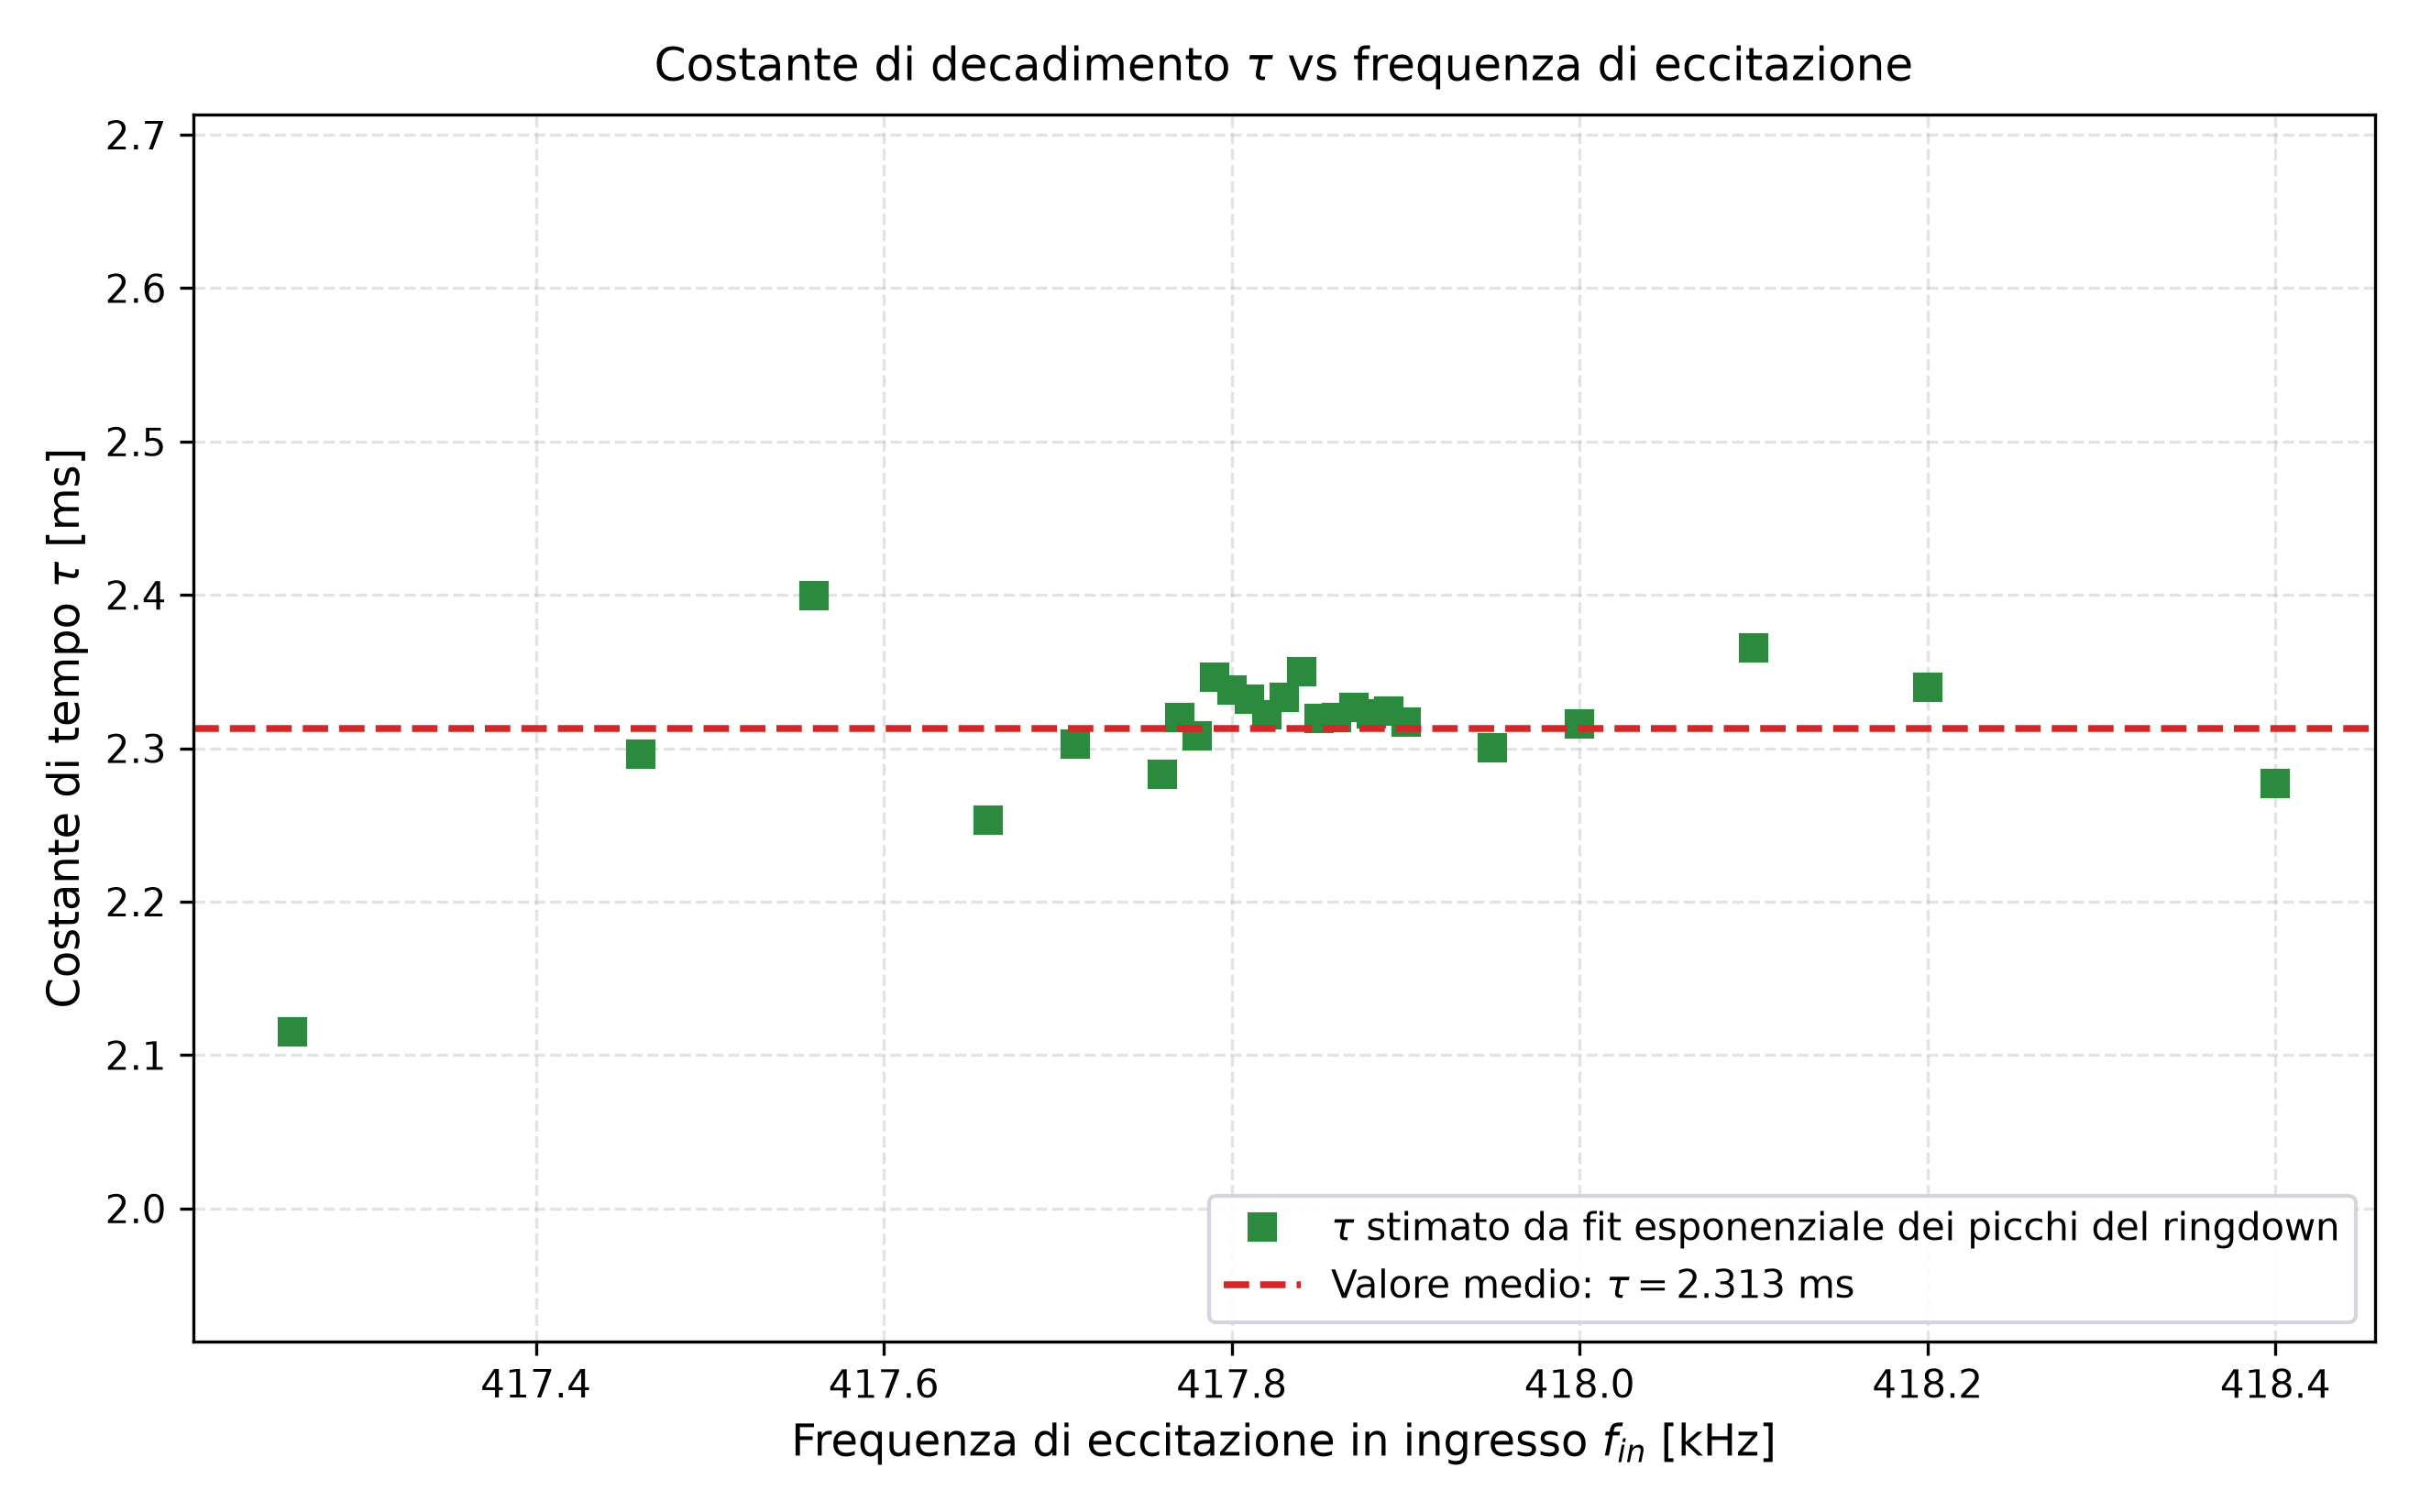
\includegraphics[height=0.88\textheight, width=0.98\textwidth, keepaspectratio]{../Ampiezza_Frequenza/grafici/tau_vs_frequenza.png}
\end{frame}

% -------------------------------------------------------------
% SLIDE 5: RISPOSTA IN FREQUENZA DEL MEMS (RLC + Cp)
% -------------------------------------------------------------
\begin{frame}
\centering
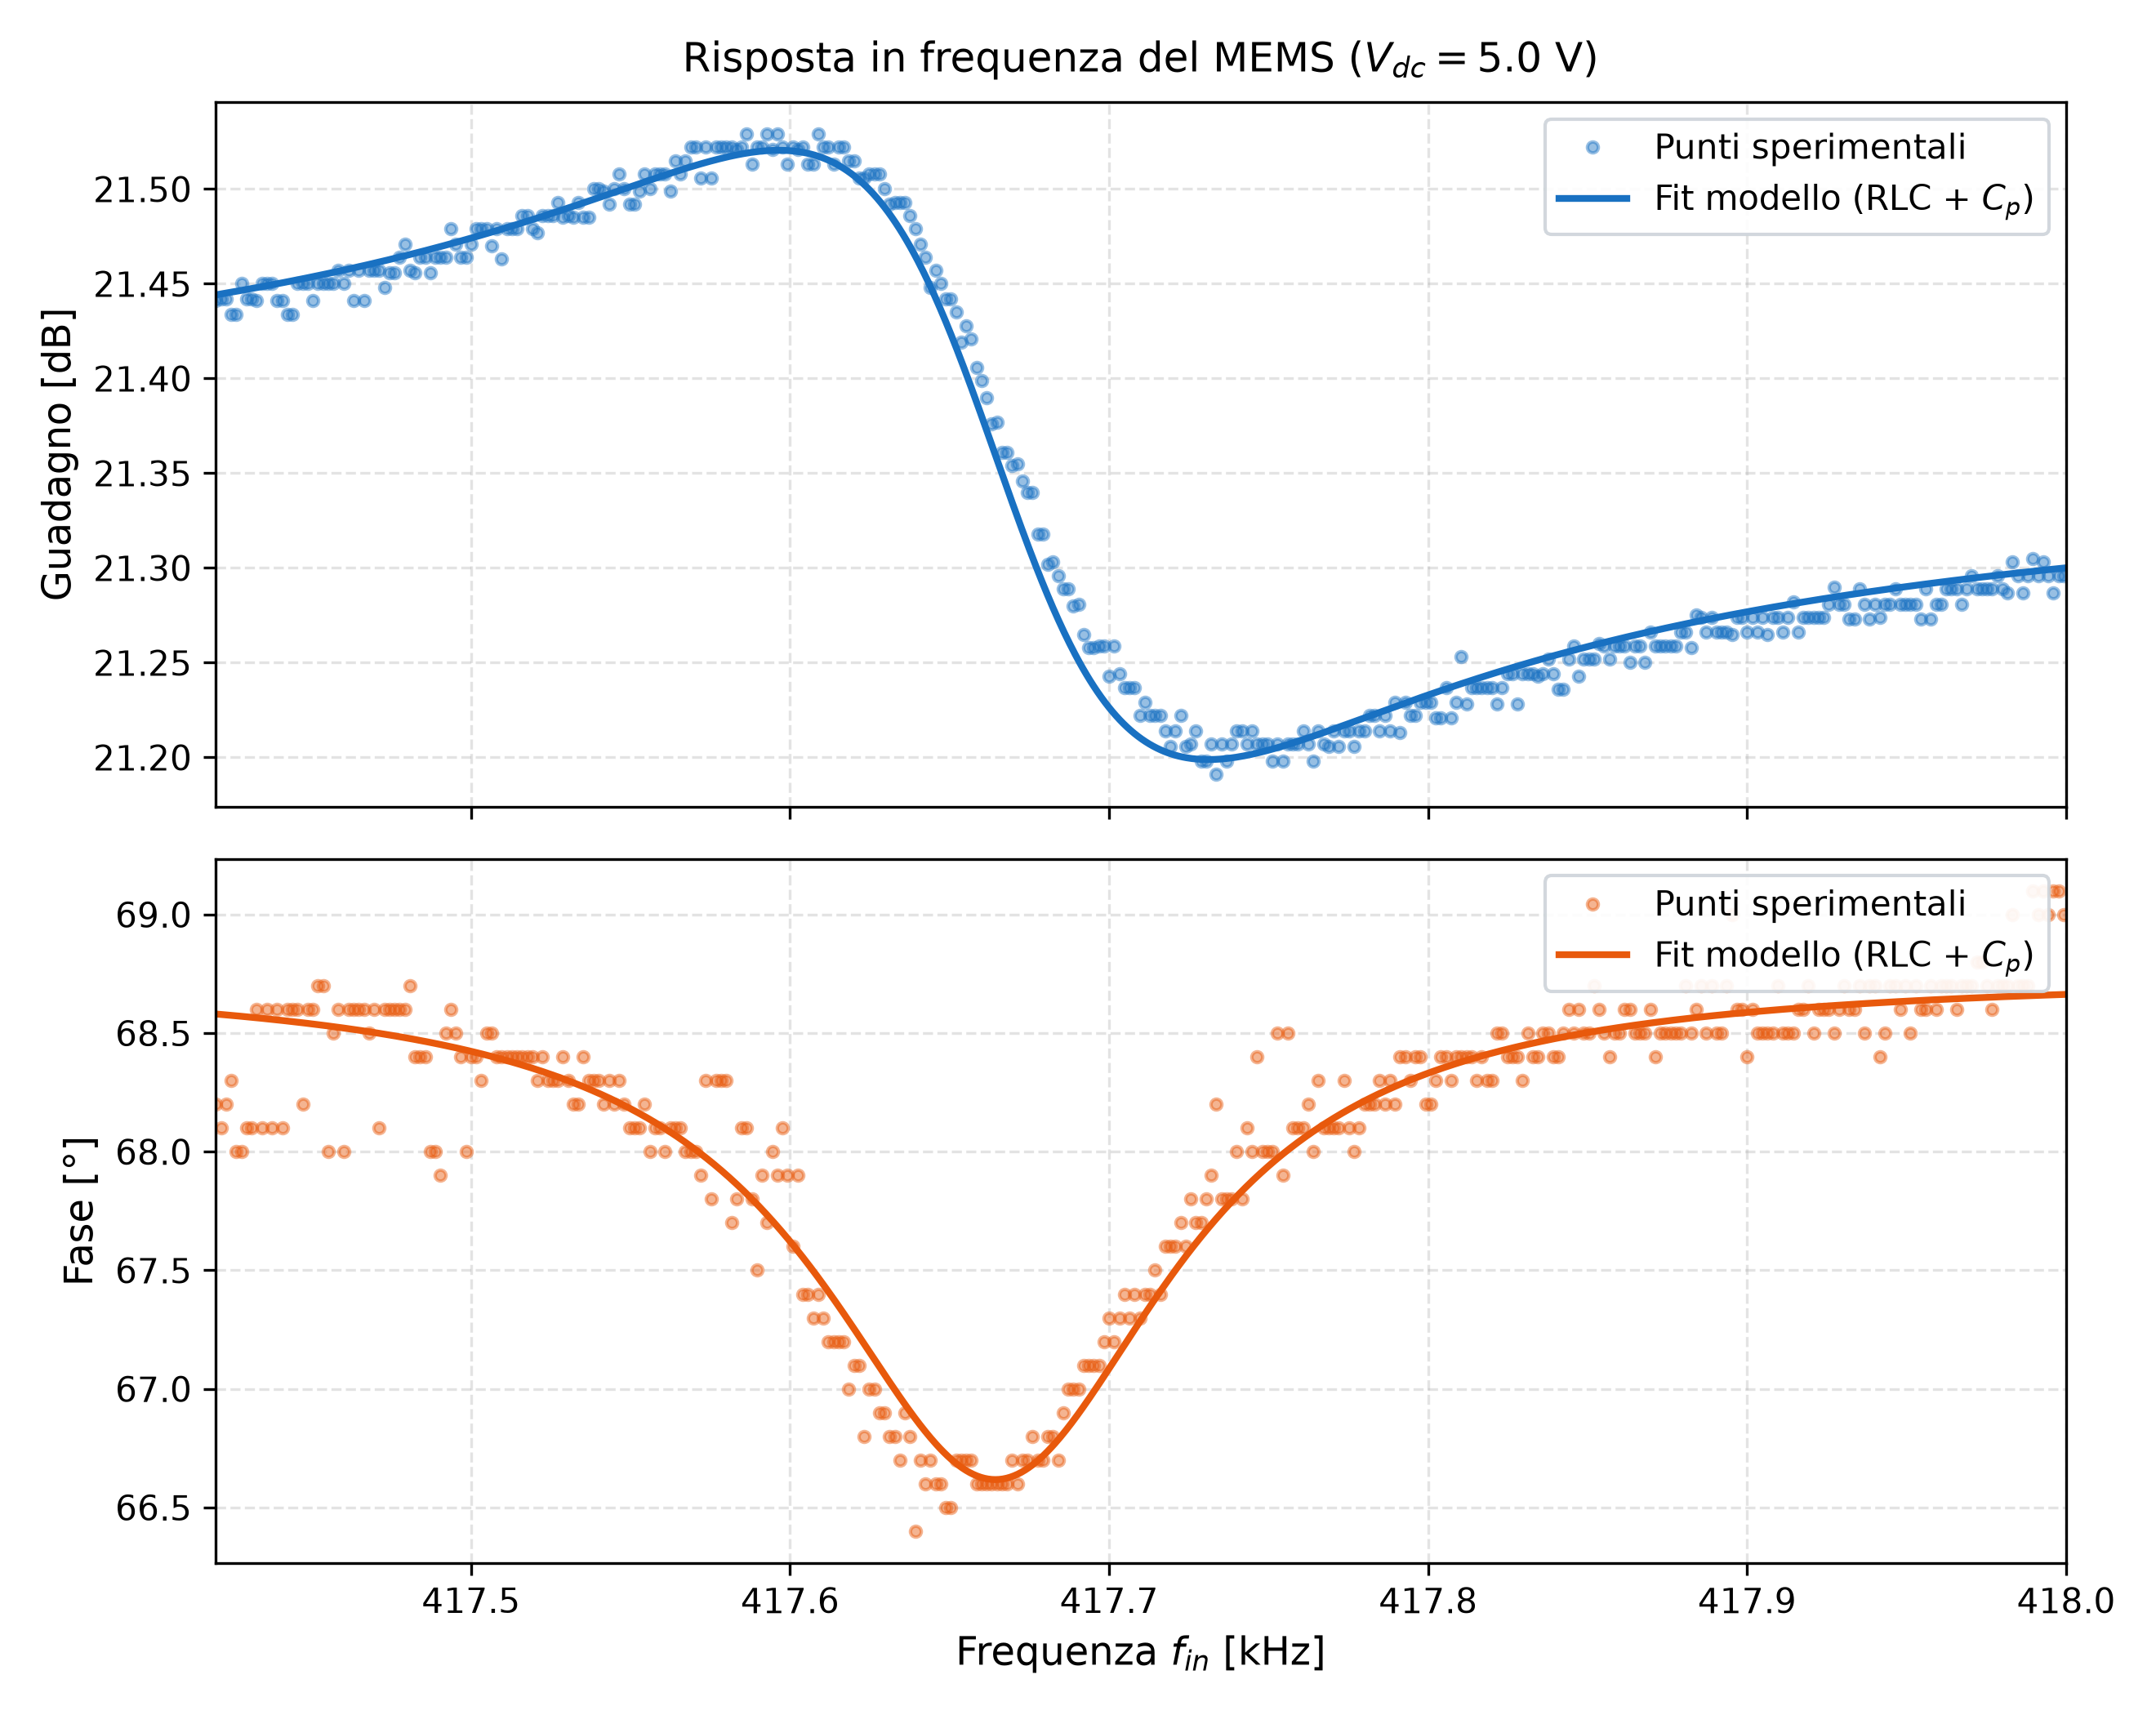
\includegraphics[height=0.88\textheight, width=0.98\textwidth, keepaspectratio]{../Risposta in frequenza/grafici/bode_completo.png}
\end{frame}

% -------------------------------------------------------------
% SLIDE 6: RISPOSTA IN FREQUENZA COMPENSATA SOFTWARE
% -------------------------------------------------------------
\begin{frame}
\centering
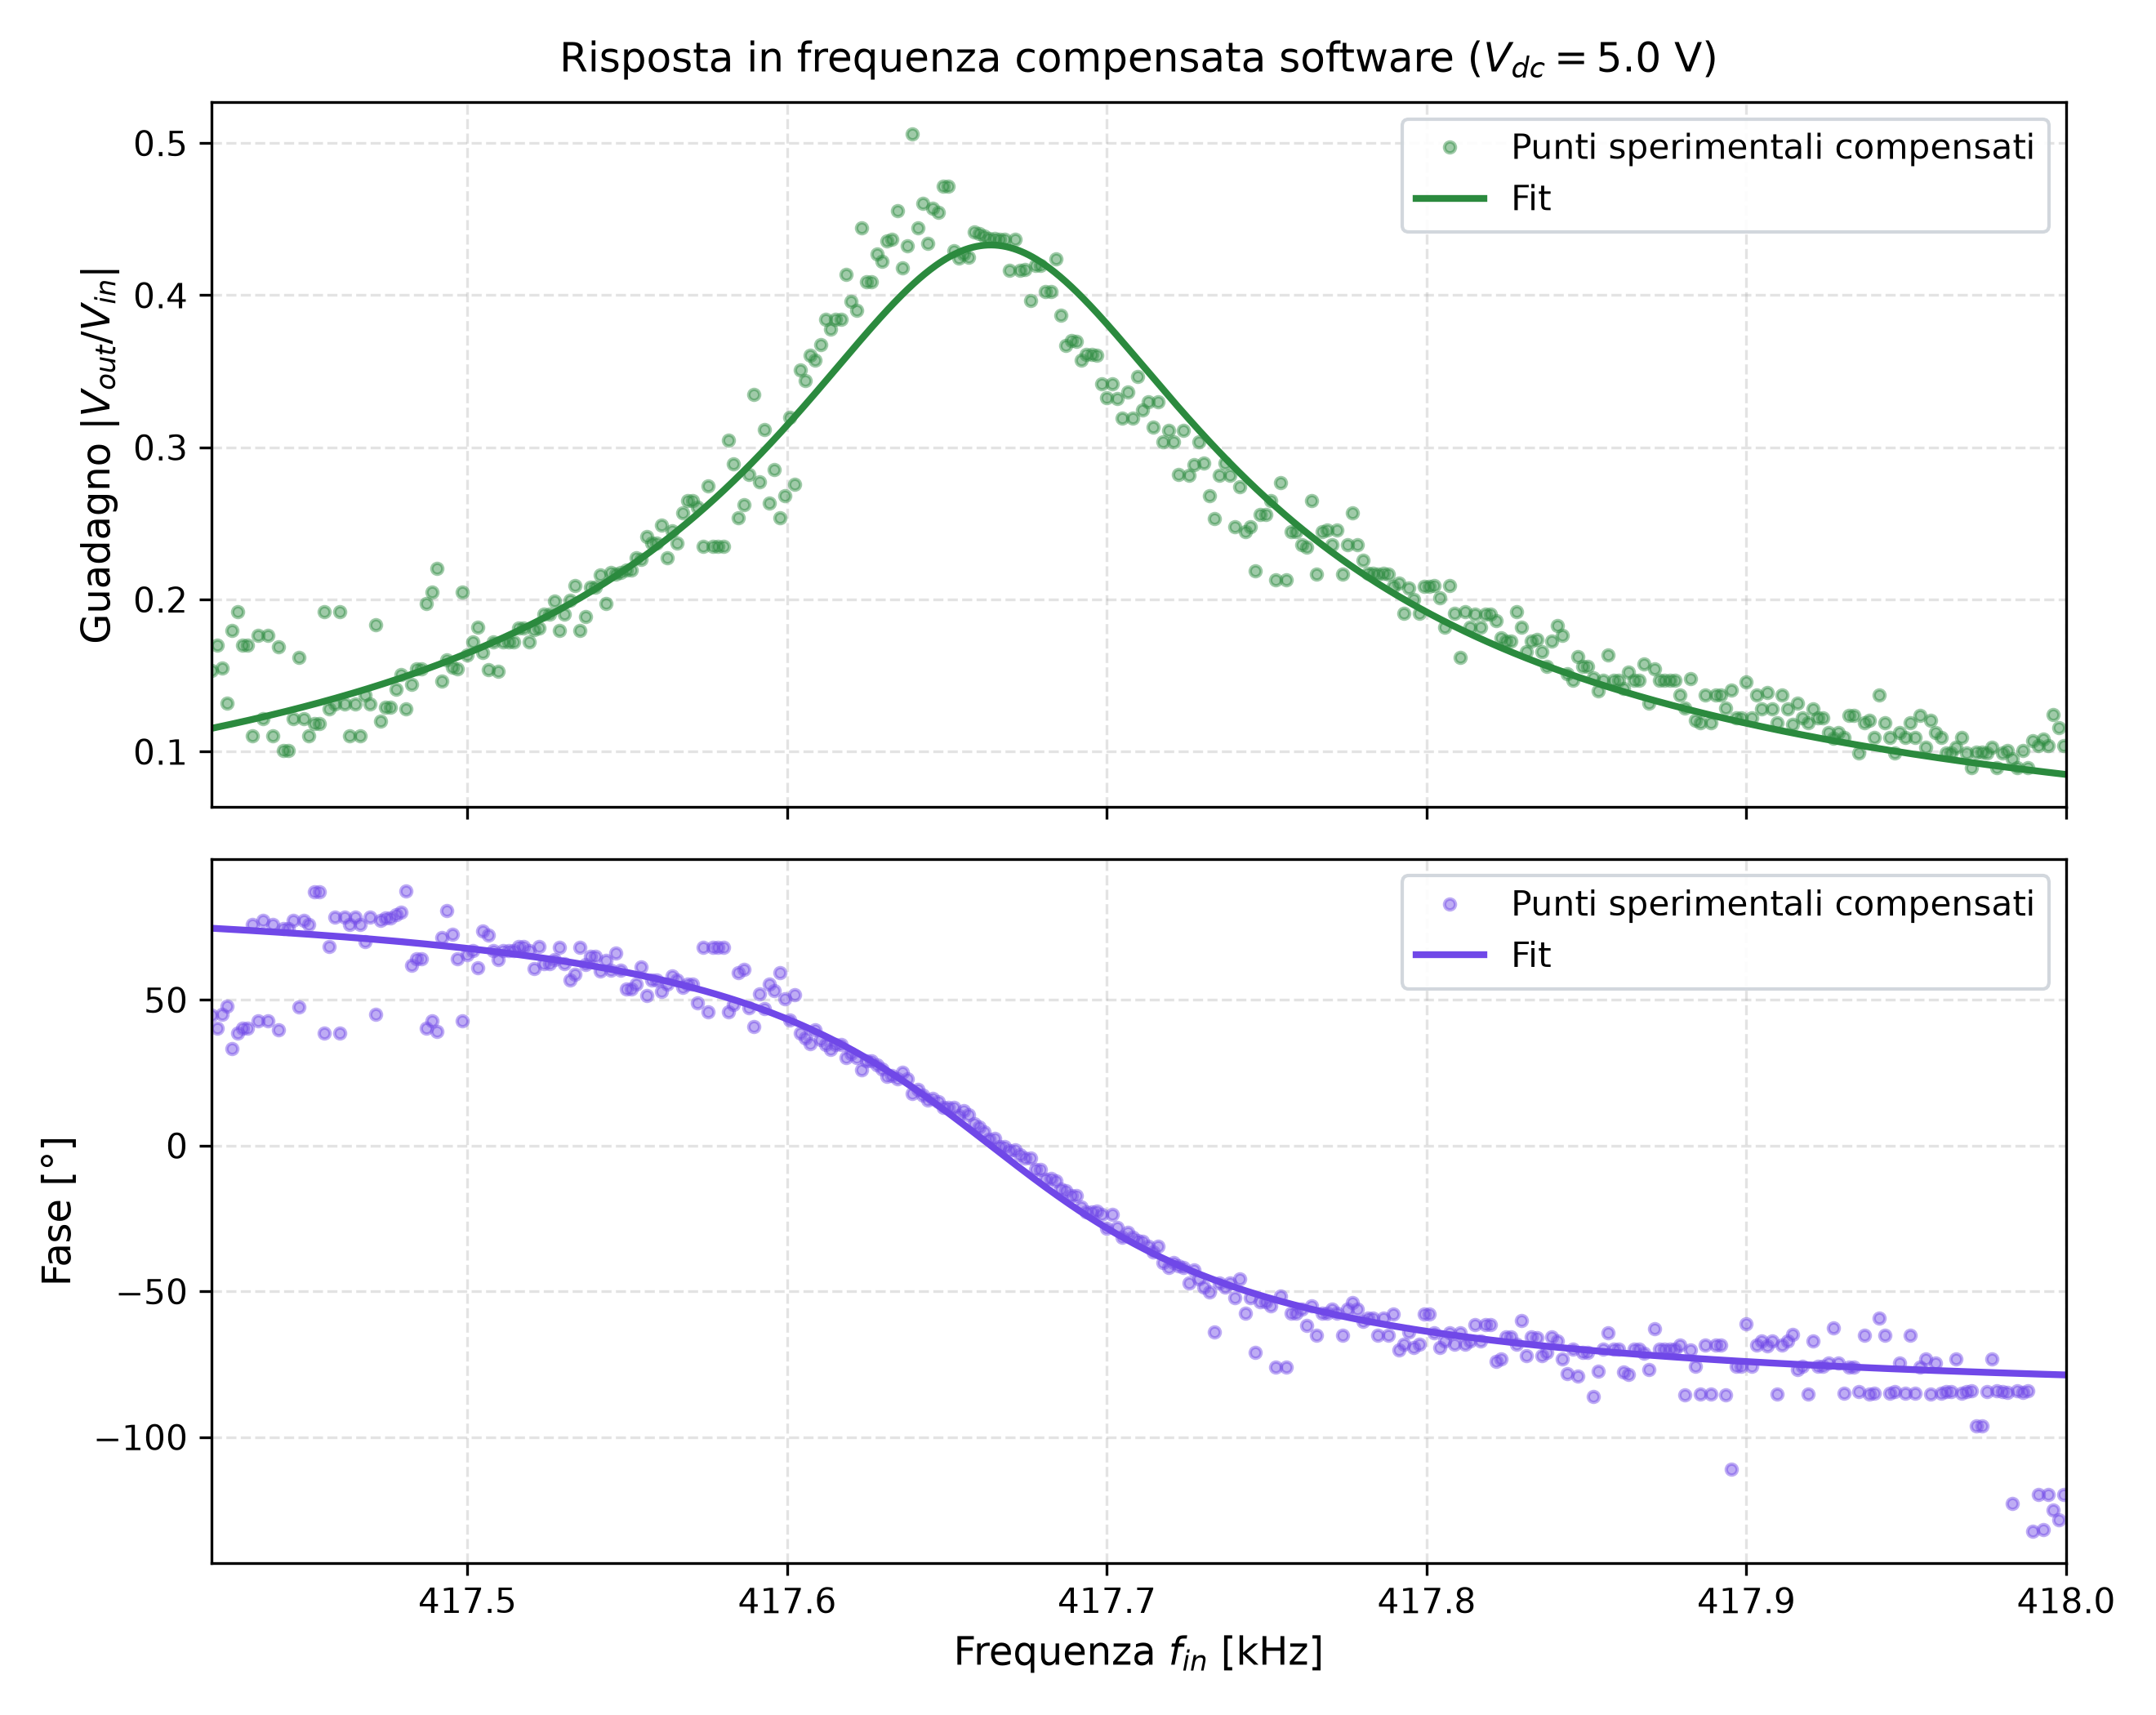
\includegraphics[height=0.88\textheight, width=0.98\textwidth, keepaspectratio]{../Risposta in frequenza/grafici/bode_compensato.png}
\end{frame}

% -------------------------------------------------------------
% SLIDE 7: EFFETTO DI SPRING SOFTENING (f1^2 vs V_DC^2)
% -------------------------------------------------------------
\begin{frame}
\centering
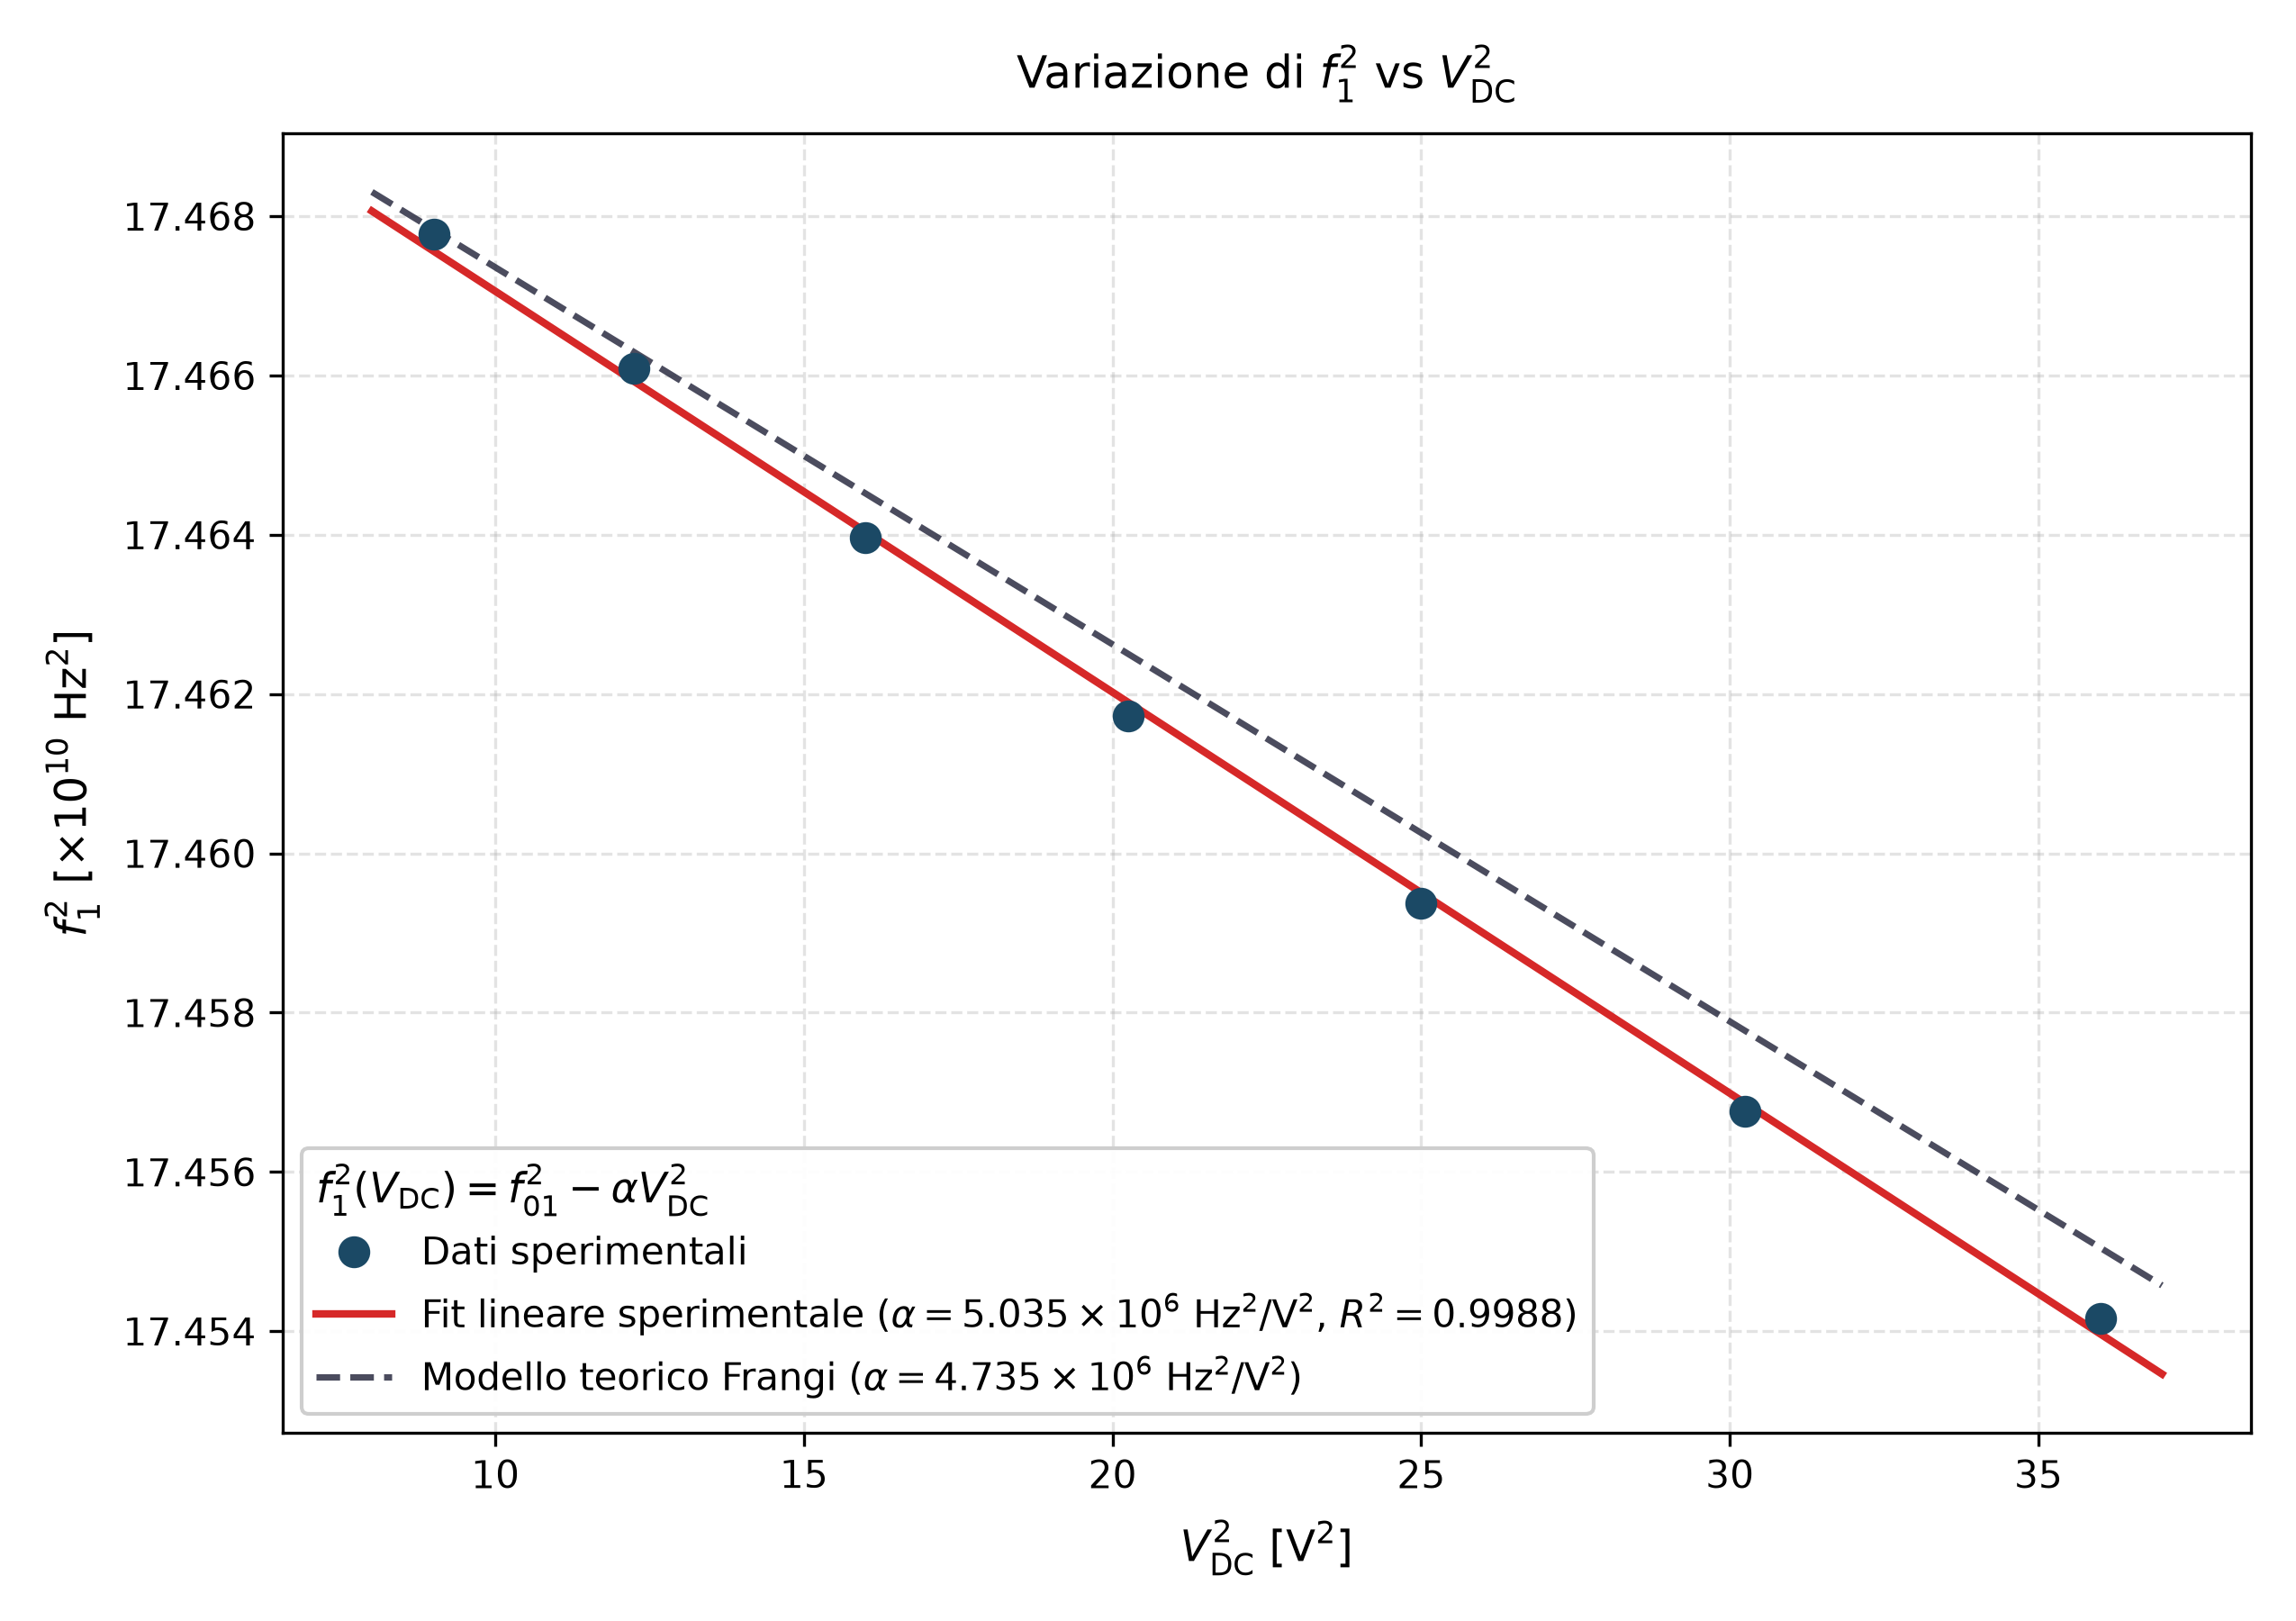
\includegraphics[height=0.84\textheight, width=0.96\textwidth, keepaspectratio]{../Frequenza_Vdc/grafici/f1_quadro_vs_vdc_quadro.png}
\end{frame}

% -------------------------------------------------------------
% SLIDE 8: GRAFICO SPERIMENTALE A SCHERMO INTERO
% -------------------------------------------------------------
\begin{frame}{Risposta allo spegnimento del gate, con capacità parassita compensata \\ ($V_{DC} = 0\text{ V}$, $A_{V_{in}} = 100\text{ mV}$, $f_{V_{in}} = 417.830\text{ kHz}$)} 
\centering
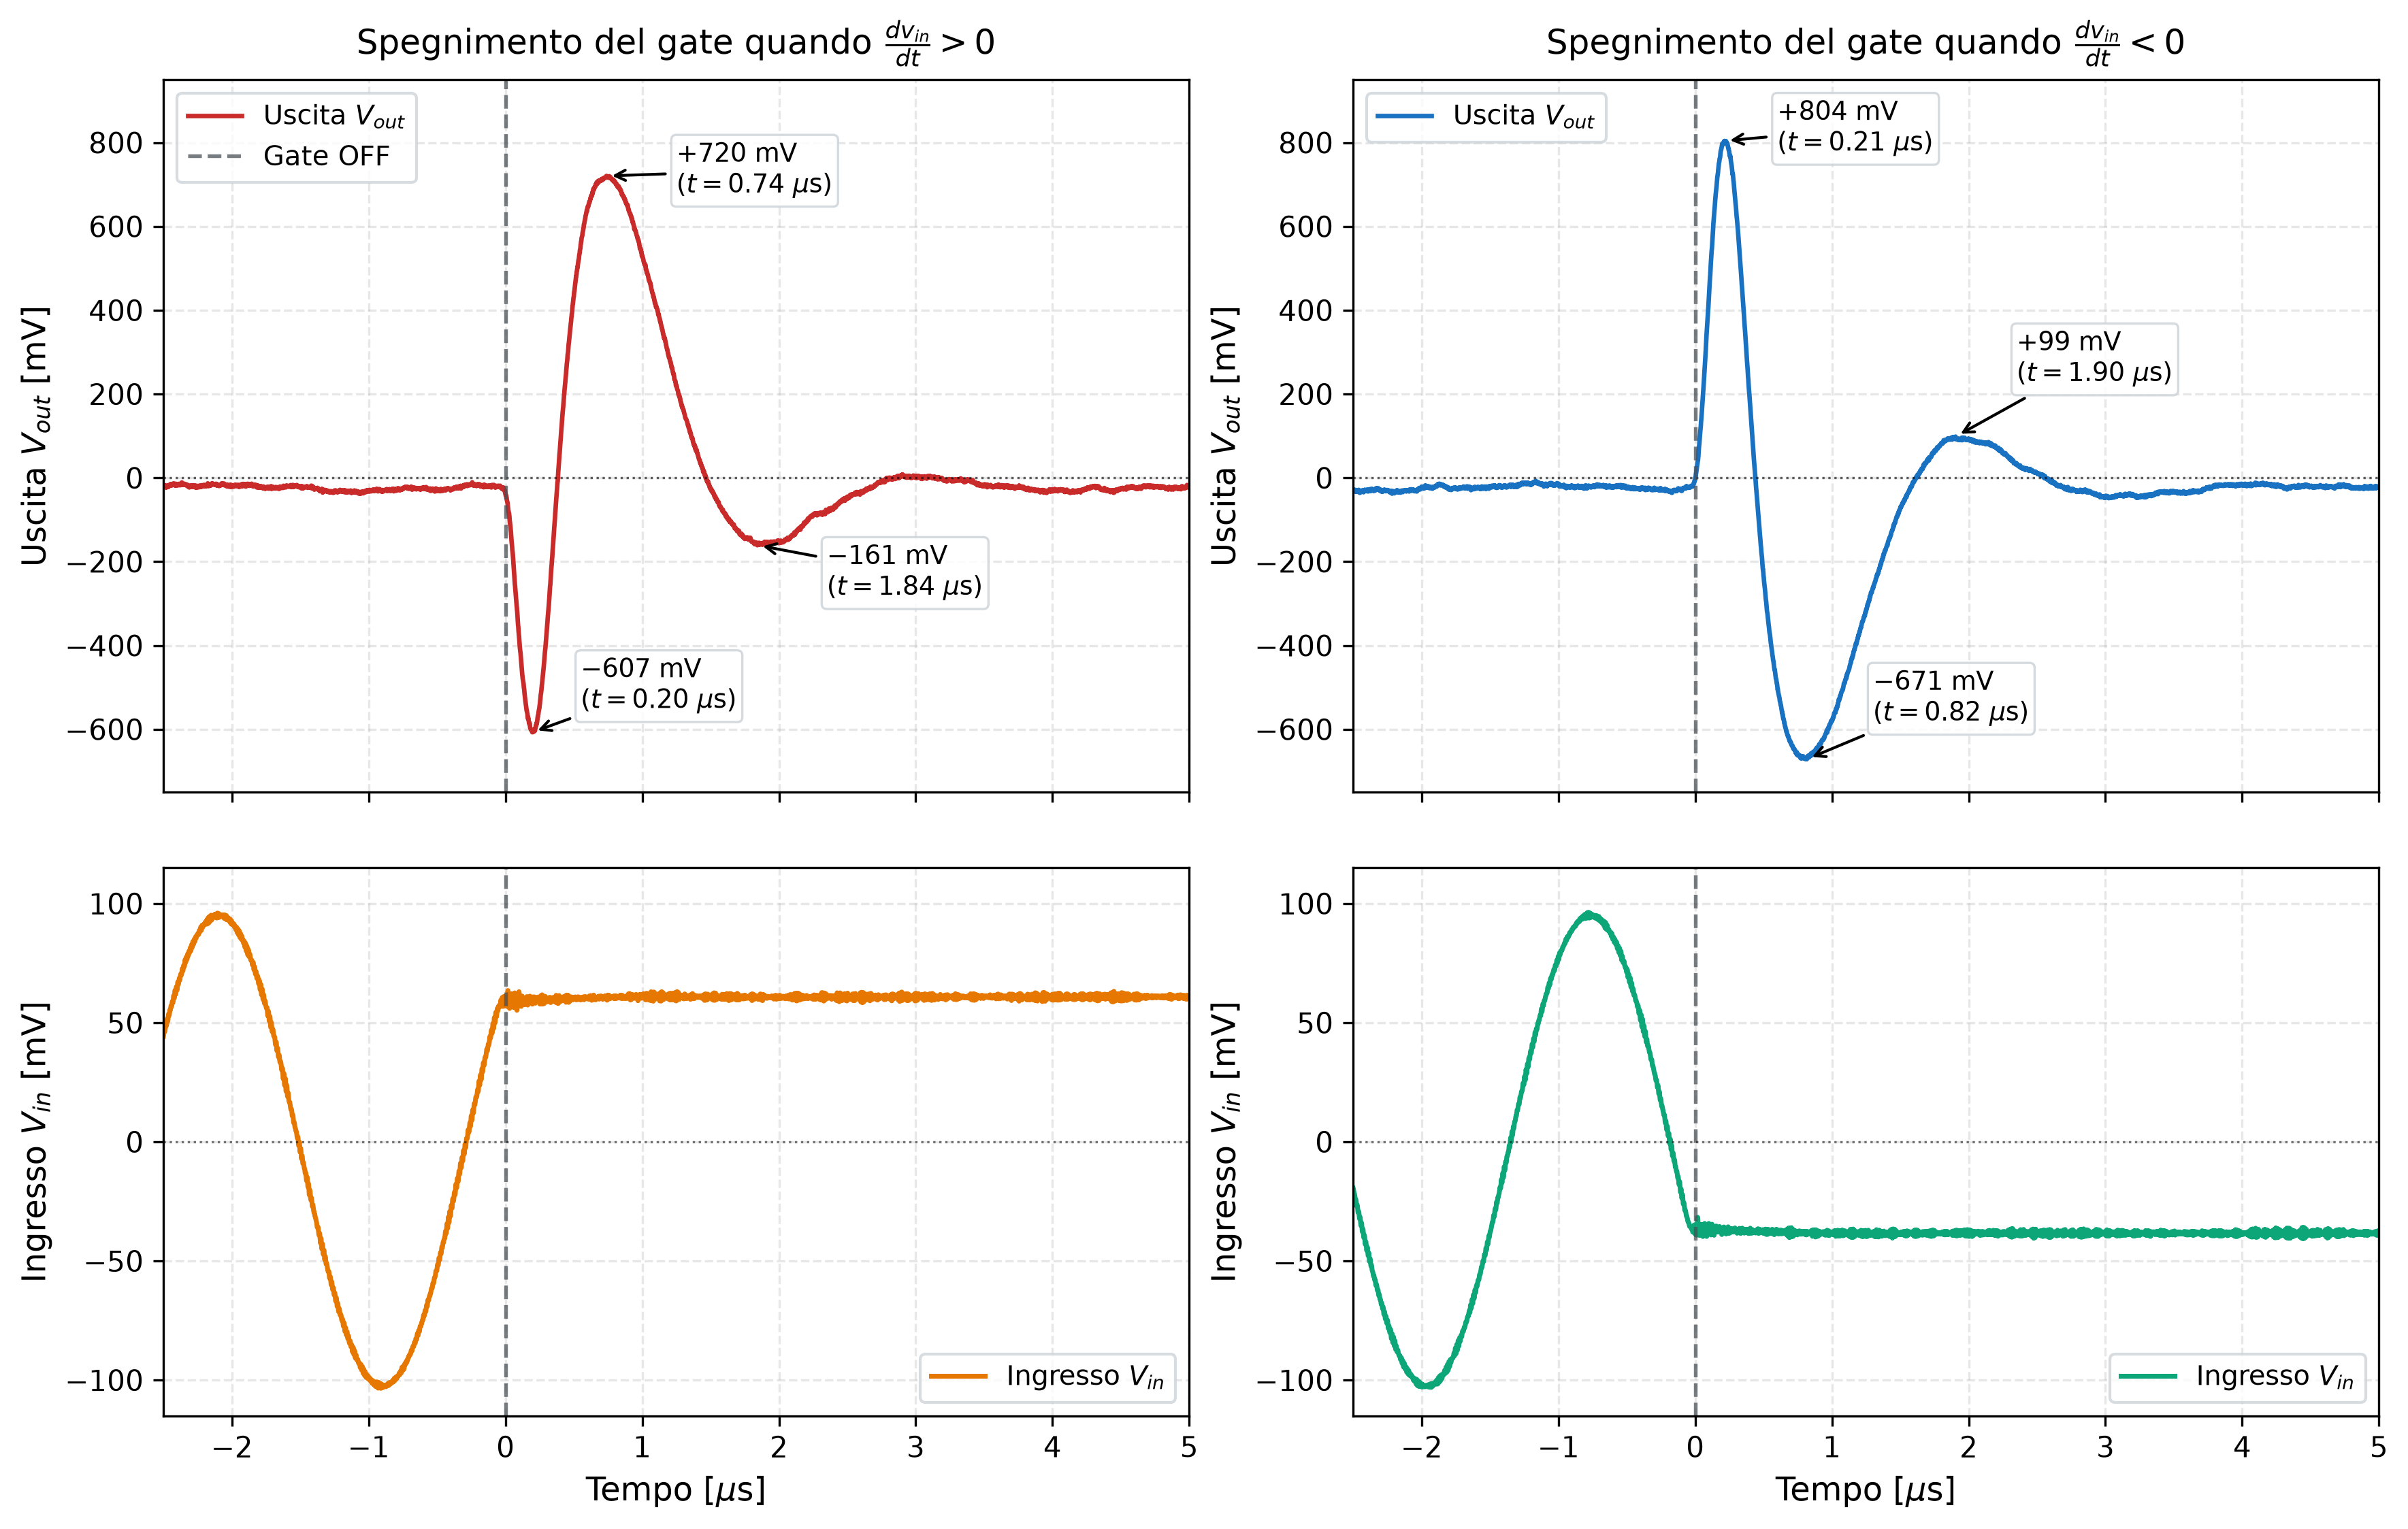
\includegraphics[height=0.77\textheight]{../Oscillazione parassita/Grafici/transitorio_elettrico_vdc0.png}
\end{frame}

% -------------------------------------------------------------
% SLIDE 9: ORIGINE DEL DISTURBO
% -------------------------------------------------------------
\begin{frame}{Origine del disturbo}
\begin{itemize}
  \setlength{\itemsep}{0.02em}
  \item Con $V_{DC} = 0\text{ V}$:
  \[
    i_{\text{RLC}}(t) \approx c_{0,DA}^{(1)} V_{DC} \dot{q}_1(t) = 0\text{ A}
  \]

  \item Corrente parassita netta iniettata al nodo d'ingresso del TIA dovuta a $\Delta C = C_p - C_c$:
  \[
    i_{\text{net}}(t) = \Delta C \frac{dv_{in}(t)}{dt}
  \]

  \item Gradino di corrente allo spegnimento del gate:
  \[
    \Delta I = 0 - i_{\text{net}}(t) = -\Delta C \frac{dv_{in}}{dt}
  \]
  \begin{itemize}
    \setlength{\itemsep}{0.1em}
    \item Pendenza negativa $\frac{dv_{in}}{dt} < 0 \implies \Delta I > 0$: picco iniziale positivo di $+804\text{ mV}$ 
    \item Pendenza positiva $\frac{dv_{in}}{dt} > 0 \implies \Delta I < 0$: picco iniziale negativo di $-607\text{ mV}$
  \end{itemize}


    \item Oscillazione parassita a $\approx 600\text{ kHz}$
    \item Scende sotto il $10\%$ del picco massimo in $\approx 2.2\ \mu\text{s}$
  \end{itemize}
\end{frame}

% -------------------------------------------------------------
% SLIDE 10: FUNZIONE DI TRASFERIMENTO COMPLESSIVA E CIRCUITO
% -------------------------------------------------------------
\begin{frame}{Modello circuitale
 \\
 (con $C_{\text{in}}$ e $C_f$ per giustificare la frequenza di oscillazione a $\approx 600\text{ kHz}$ e  lo smorzamento)}
\centering
\begin{circuitikz}[scale=0.68, transform shape, line width=0.7pt]
  % Ingresso Vin
  \draw (-1.2, 0.5) node[left] {$v_{in}(t)$} to[short, o-] (-0.2, 0.5);
  \draw (-0.2, 0.5) -- (-0.2, 1.6);
  \draw (-0.2, 0.5) -- (-0.2, -0.6);
  
  % Ramo parassita diretto Cp (in alto)
  \draw (-0.2, 1.6) to[C, l_={$C_p$}] (3.6, 1.6) -- (4.0, 1.6);

  % Ramo compensazione con blocco [-1] e Cc (in basso)
  \node[draw, rectangle, fill=white, inner sep=3.8pt, font=\scriptsize] (inv) at (1.0, -0.6) {$-1$};
  \draw (-0.2, -0.6) -- (inv.west);
  \draw (inv.east) -- (1.7, -0.6) to[C, l={$C_c$}] (3.6, -0.6) -- (4.0, -0.6);

  % Connessione al nodo di sense
  \draw (4.0, 1.6) -- (4.0, -0.6);
  \draw (4.0, 0.5) to[short, -*] (5.0, 0.5) coordinate (sense);
  
  % Cin verso massa (etichetta in basso a sinistra in ampio spazio vuoto)
  \draw (5.0, 0.5) to[C, *-] (5.0, -1.4) node[ground]{};
  \node[left=3pt] at (4.8, -0.85) {$C_{\text{in}}$};

  % TIA OPA656 (distanziato da Cin per massima chiarezza visiva)
  \node[op amp] (opamp1) at (7.2, 0) {};
  \node[font=\scriptsize, below=3pt] at (opamp1.south) {OPA656};
  \draw (sense) -- (opamp1.-);
  \draw (opamp1.+) -- (opamp1.+ |- 0, -1.4) node[ground]{};

  % Retroazione TIA (Cf sopra Rf)
  \draw (sense) -- (5.0, 2.3) -- (5.7, 2.3);
  \draw (5.7, 3.0) to[C, l=$C_f$] (7.9, 3.0);
  \draw (5.7, 1.8) to[R, l=$R_f$] (7.9, 1.8);
  \draw (5.7, 3.0) -- (5.7, 1.8);
  \draw (7.9, 3.0) -- (7.9, 1.8);
  \draw (7.9, 2.3) -| (opamp1.out);

  % Secondo stadio AD817 (invertente G = -10)
  \node[op amp] (opamp2) at (11.5, -0.5) {};
  \node[font=\scriptsize, below=3pt] at (opamp2.south) {AD817};
  \draw (opamp1.out) -- (8.4, 0) to[R, l_={$R_1$}] (10.2, 0) -- (opamp2.-);
  \draw (opamp2.+) -- (opamp2.+ |- 0, -1.4) node[ground]{};

  % Retroazione AD817 (R2)
  \draw (opamp2.-) to[short, *-] ++(0, 1.5) to[R, l={$R_2$}] ++(2.0, 0) -| (opamp2.out);
  
  % Uscita finale
  \draw (opamp2.out) to[short, -o] ++(0.8, 0) node[right] {$V_{\text{out}}$};
\end{circuitikz}

\vspace{0.4em}
{\small
Modellando l'operazionale OPA656 con guadagno $A(s) \approx \frac{\omega_t}{s} \implies V^- = -\frac{s}{\omega_t} V_{\text{out}_{\text{TIA}}}$
}

\vspace{0.1em}
\[
  \frac{V_{\text{out}}(s)}{V_{in}(s)} = \frac{10 \cdot s R_f (C_p - C_c)}{1 + s \left( R_f C_f + \frac{1}{\omega_t} \right) + s^2 \frac{R_f (C_{\text{in}} + C_p + C_c + C_f)}{\omega_t}}
\]
\end{frame}

% -------------------------------------------------------------
% SLIDE 11: SOVRAPPOSIZIONE MISURA REALE VS MODELLO TEORICO
% -------------------------------------------------------------
\begin{frame}{Simulazione del transistorio}
\begin{columns}[c]
  \begin{column}{0.63\textwidth}
    \centering
    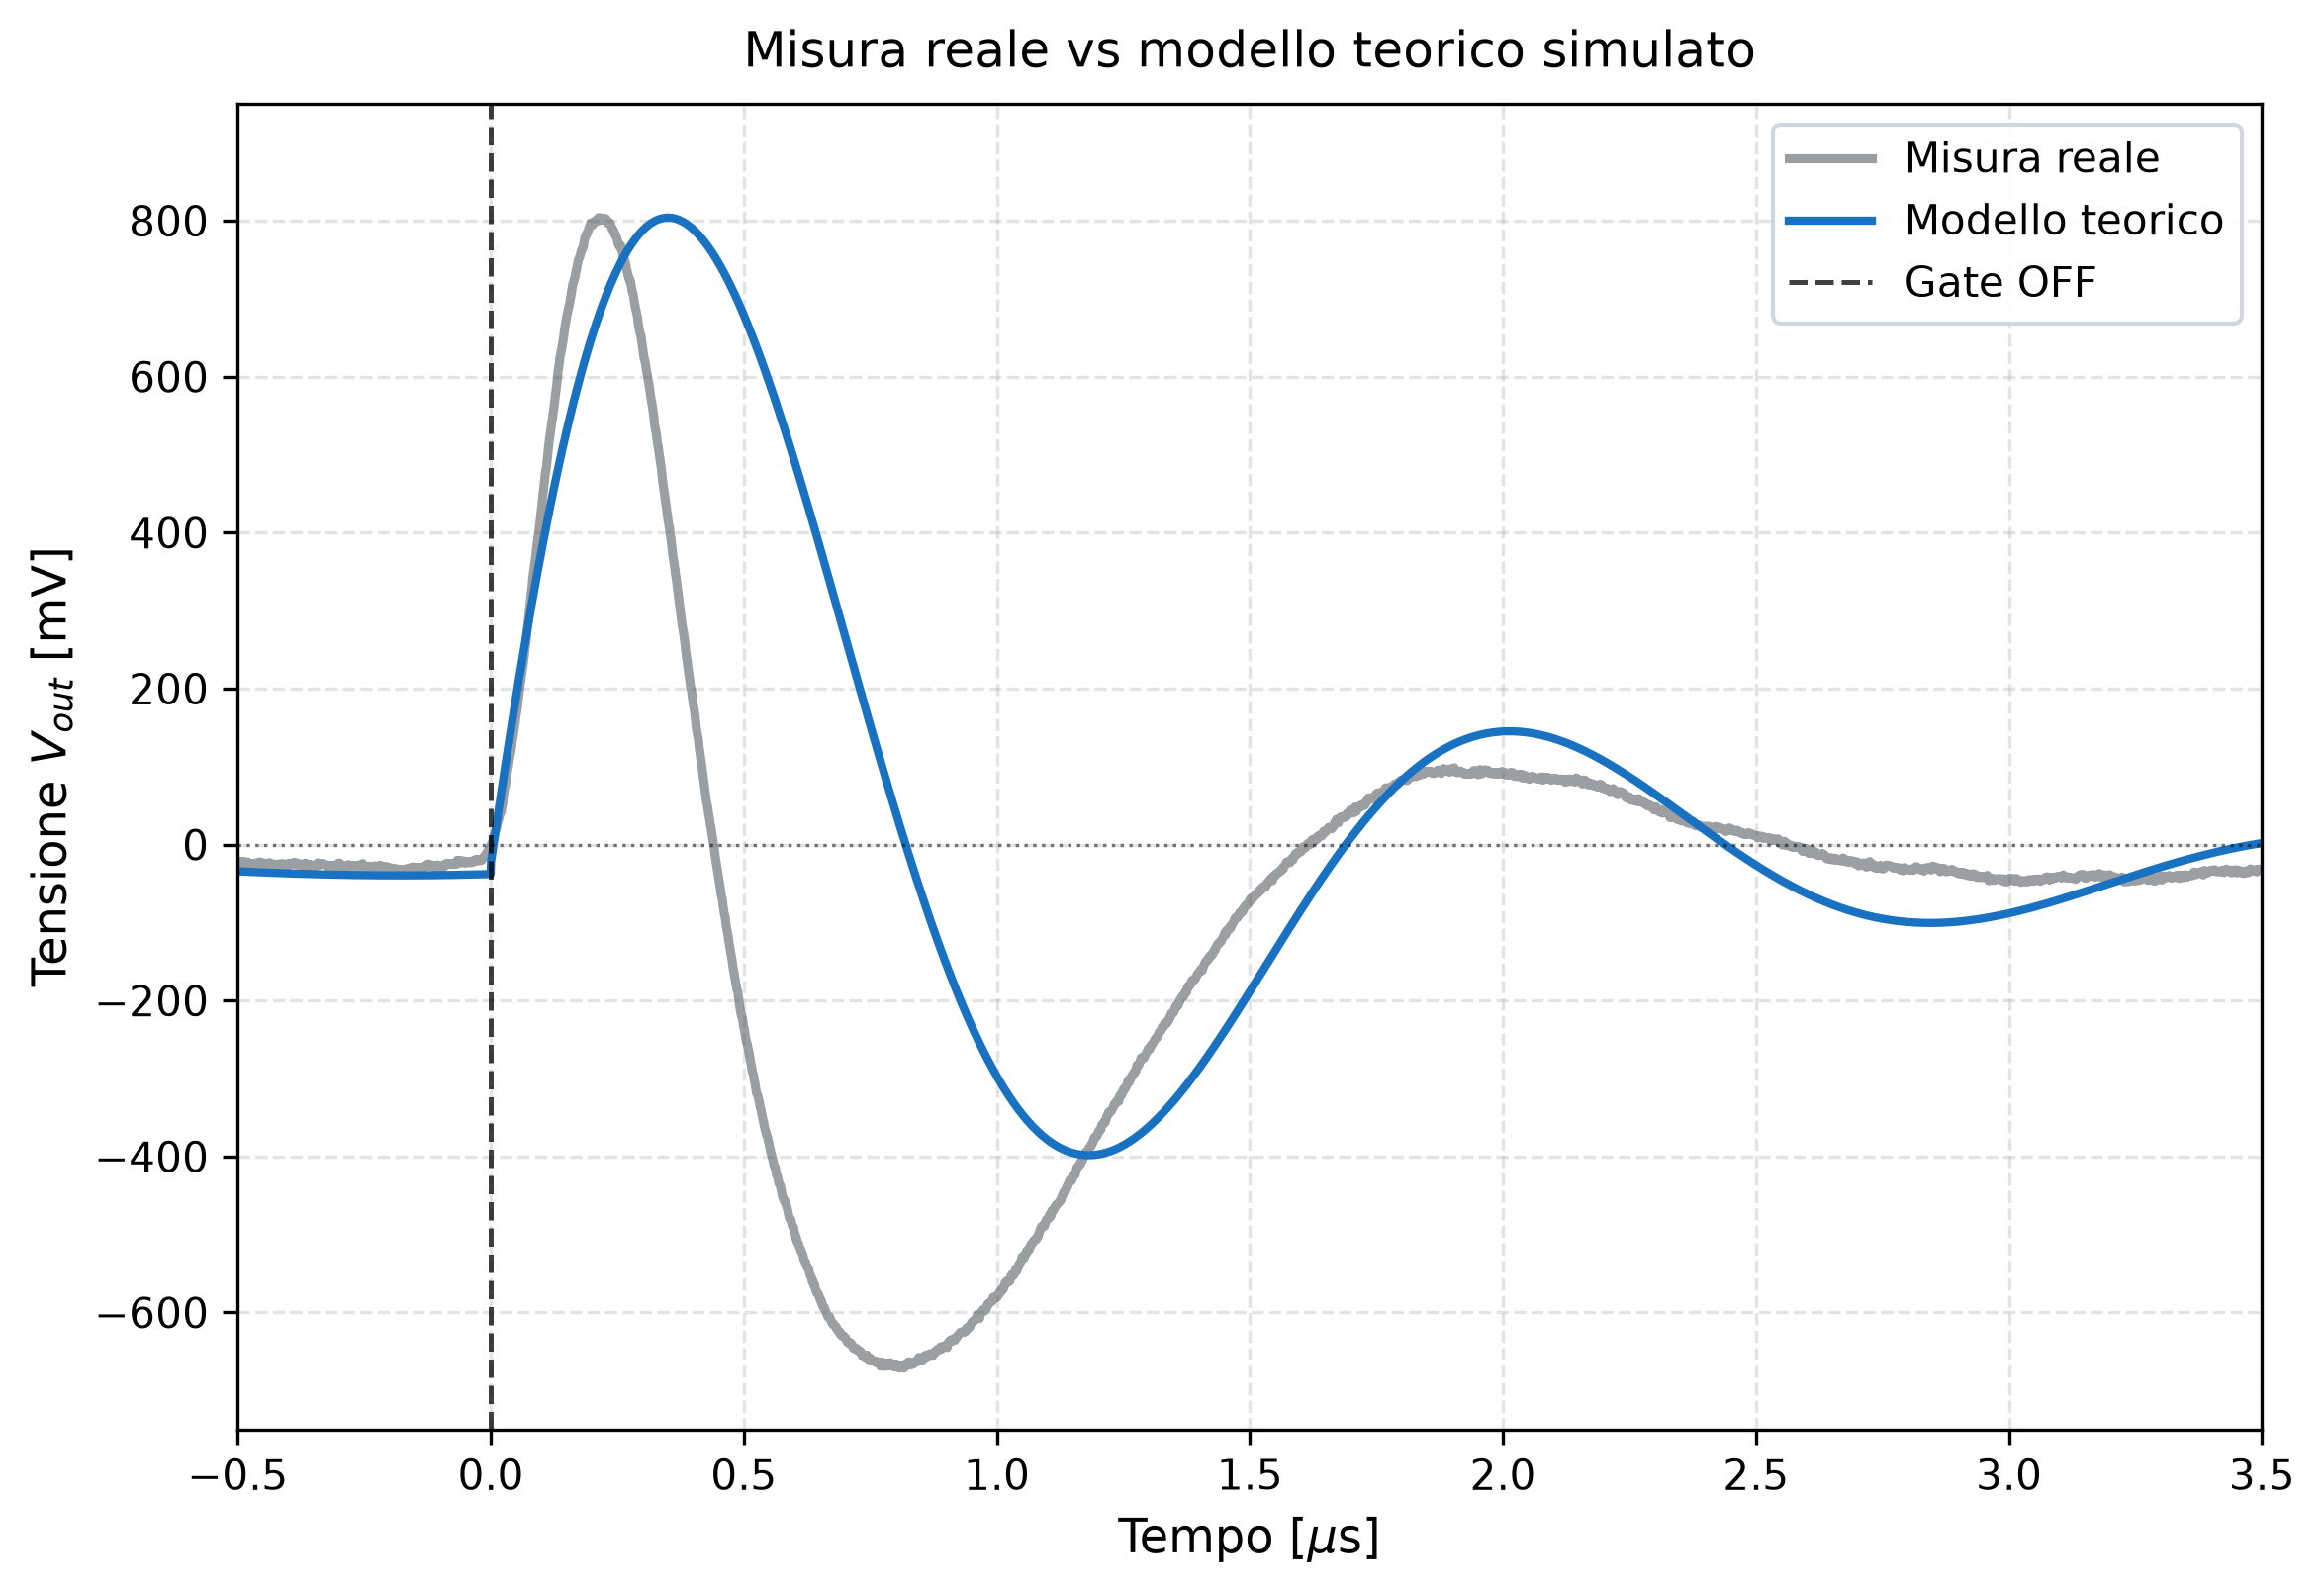
\includegraphics[width=\linewidth]{../Oscillazione parassita/Grafici/sovrapposizione_simulazione_reale.png}
  \end{column}
  \begin{column}{0.35\textwidth}
    \centering
    \footnotesize
    \begin{tabular}{ll}
      \toprule
      Parametro & Valore \\
      \midrule
      $R_f$ & $500\text{ k}\Omega$ \\
      $C_{\text{in}}$ & $188\text{ pF}$ \\
      $C_f$ & $0.25\text{ pF}$ \\
      $C_p, C_c$ & $\approx 1.0\text{ pF}$ \\
      $\Delta C$ & $C_p - C_c \approx 40\text{ fF}$ \\
      $\omega_t$ & $1.445\times 10^9\text{ rad/s}$ \\
      $G_2$ & $-10$ \\
      \bottomrule
    \end{tabular}
  \end{column}
\end{columns}
\end{frame}

% -------------------------------------------------------------
% SLIDE 12: VARIAZIONE DEI PICCHI VS FASE DI SPEGNIMENTO GATE
% -------------------------------------------------------------
\begin{frame}{Variazione dei picchi dell'oscillazione con la fase di spegnimento del gate}
  \centering
  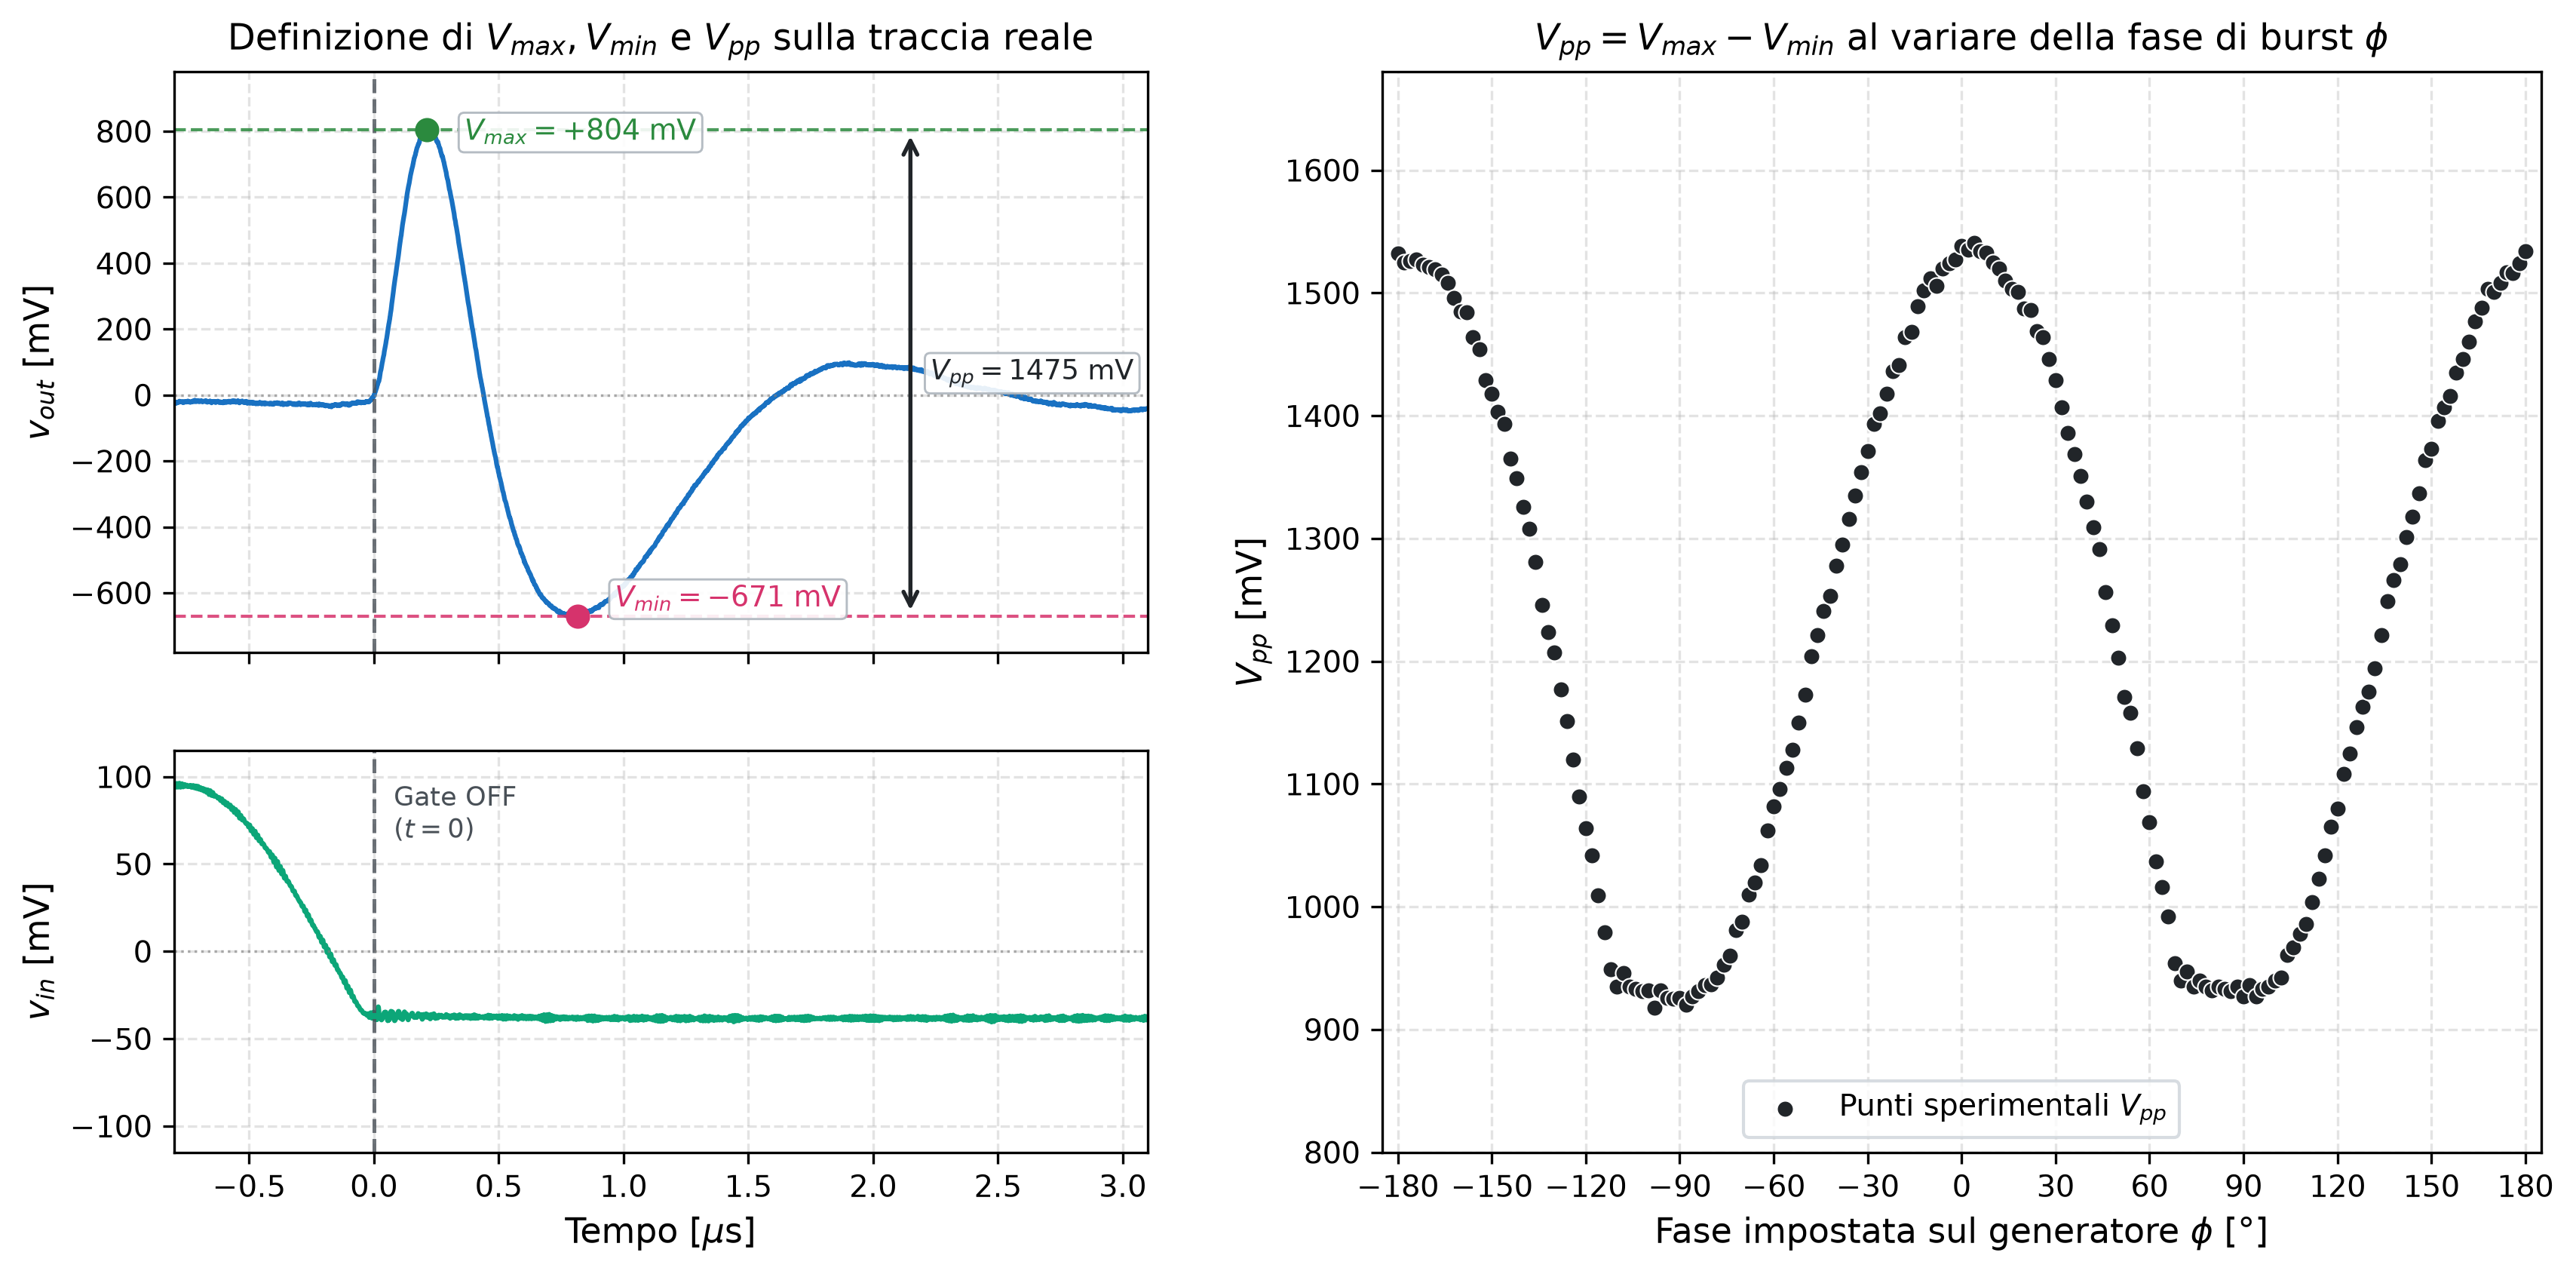
\includegraphics[height=0.76\textheight]{../Oscillazione parassita/Grafici/sweep_fase_con_scope.png}
\end{frame}

\end{document}
